%
% Niniejszy plik stanowi przykład formatowania pracy magisterskiej na
% Wydziale MIM UW.  Szkielet użytych poleceń można wykorzystywać do
% woli, np. formatujac wlasna prace.
%
% Zawartosc merytoryczna stanowi oryginalnosiagniecie
% naukowosciowe Marcina Wolinskiego.  Wszelkie prawa zastrzeżone.
%
% Copyright (c) 2001 by Marcin Woliński <M.Wolinski@gust.org.pl>
% Poprawki spowodowane zmianami przepisów - Marcin Szczuka, 1.10.2004
% Poprawki spowodowane zmianami przepisow i ujednolicenie 
% - Seweryn Karłowicz, 05.05.2006
% Dodanie wielu autorów i tłumaczenia na angielski - Kuba Pochrybniak, 29.11.2016

% dodaj opcję [licencjacka] dla pracy licencjackiej
% dodaj opcję [en] dla wersji angielskiej (mogą być obie: [licencjacka,en])
\documentclass[licencjacka]{pracamgr}


% Dane magistranta:
\autor{Mateusz Kiebała}{359758}

\title{Biblioteka do implementacji algorytmów minimalnych}
%\tytulang{A library for implementing minimal algoritms}

%kierunek: 
\kierunek{informatyka}

% informatyka - nie okreslamy zakresu (opcja zakomentowana)
% matematyka - zakres moze pozostac nieokreslony,
% a jesli ma byc okreslony dla pracy mgr,
% to przyjmuje jedna z wartosci:
% {metod matematycznych w finansach}
% {metod matematycznych w ubezpieczeniach}
% {matematyki stosowanej}
% {nauczania matematyki}
% Dla pracy licencjackiej mamy natomiast
% mozliwosc wpisania takiej wartosci zakresu:
% {Jednoczesnych Studiow Ekonomiczno--Matematycznych}

% \zakres{Tu wpisac, jesli trzeba, jedna z opcji podanych wyzej}

% Praca wykonana pod kierunkiem:
% (podać tytuł/stopień imię i nazwisko opiekuna
% Instytut
% ew. Wydział ew. Uczelnia (jeżeli nie MIM UW))
\opiekun{dr. Jacka Sroki}

% miesiąc i~rok:
\date{Czerwiec 2019}

%Podać dziedzinę wg klasyfikacji Socrates-Erasmus:
\dziedzina{ 
%11.0 Matematyka, Informatyka:\\ 
%11.1 Matematyka\\ 
%11.2 Statystyka\\ 
11.3 Informatyka\\
%11.4 Sztuczna inteligencja\\ 
%11.5 Nauki aktuarialne\\
%11.9 Inne nauki matematyczne i informatyczne
}

%Klasyfikacja tematyczna wedlug AMS (matematyka) lub ACM (informatyka)
\klasyfikacja{412521 Programy i oprogramowanie użytkowe. Biblioteki programów}

% Słowa kluczowe:
\keywords{Spark, Hadoop, MapReduce, algorytmy minimalne, algorytmy równoległe, programowanie rozproszone, TeraSort, big data}

% Tu jest dobre miejsce na Twoje własne makra i~środowiska:
\newtheorem{defi}{Definicja}[section]
\usepackage{graphicx}
\usepackage{tabularx,ragged2e,booktabs,caption}
\usepackage{algpseudocode}
\usepackage{float}
\usepackage{listings}
\usepackage{xcolor}

\colorlet{punct}{red!60!black}
\definecolor{background}{HTML}{EEEEEE}
\definecolor{delim}{RGB}{20,105,176}
\colorlet{numb}{magenta!60!black}

\lstdefinelanguage{json}{
    basicstyle=\normalfont\ttfamily,
    numbers=left,
    numberstyle=\scriptsize,
    stepnumber=1,
    numbersep=8pt,
    showstringspaces=false,
    breaklines=true,
    frame=lines,
    backgroundcolor=\color{background},
    literate=
     *{0}{{{\color{numb}0}}}{1}
      {1}{{{\color{numb}1}}}{1}
      {2}{{{\color{numb}2}}}{1}
      {3}{{{\color{numb}3}}}{1}
      {4}{{{\color{numb}4}}}{1}
      {5}{{{\color{numb}5}}}{1}
      {6}{{{\color{numb}6}}}{1}
      {7}{{{\color{numb}7}}}{1}
      {8}{{{\color{numb}8}}}{1}
      {9}{{{\color{numb}9}}}{1}
      {:}{{{\color{punct}{:}}}}{1}
      {,}{{{\color{punct}{,}}}}{1}
      {\{}{{{\color{delim}{\{}}}}{1}
      {\}}{{{\color{delim}{\}}}}}{1}
      {[}{{{\color{delim}{[}}}}{1}
      {]}{{{\color{delim}{]}}}}{1},
}
\graphicspath{ {./} }

% koniec definicji

\begin{document}

\maketitle

%tu idzie streszczenie na strone poczatkowa
\begin{abstract}
 W ramach pracy magisterskiej została stworzona biblioteka umożliwiająca implementowanie równoległych algorytmów minimalnych. Wspiera ona dwa główne frameworki służące do pisania programów rozproszonych: Hadoop i Spark. Celem biblioteki jest udostępnienie API umożliwiającego optymalne i łatwe implementowanie algorytmów minimalnych. W ramach pracy powstały również implementacje przykładowych algorytmów minimalnych takich jak: tworzenie rankingu, statystyki prefiksowe, grupowanie, pół-złączenia (ang. \textit{semi-join}) oraz statystyka okienkowa (ang. \textit{sliding aggregation}).
\end{abstract}

\tableofcontents
%\listoffigures
%\listoftables

\chapter{Wprowadzenie}
\addcontentsline{toc}{chapter}{Wprowadzenie}

W obecnych czasach programowanie rozproszone jest prężnie rozwijającą się dziedziną informatyki. Rozwój technologii i nauki doprowadził do gwałtownego wzrostu ilości danych w różnych dziedzinach życia. Rodzi to potrzebę efektywnego przetwarzania ogromnych zbiorów informacji \cite{watson2014tutorial, wu2013data}.

Obecnie dwoma najbardziej popularnymi frameworkami do przetwarzania dużych danych są Hadoop i Spark. Pierwszy z nich opiera się na paradygmacie MapReduce, natomiast drugi jest kolekcją rozproszonych danych ze zbiorem typowych operatorów do ich przetwarzania. W obu systemach algorytm rozproszony uruchamiany jest na grupie niezależnych maszyn, komunikujących się jedynie za pomocą sieci, zwanych klastrem obliczeniowym.

Algorytm oparty o paradygmat MapReduce wykonuje się w rundach, a każda runda składa się z trzech faz: \textit{map}, \textit{shuffle} i \textit{reduce}. Podczas faz \textit{map} i \textit{reduce} nie występuje komunikacja między maszynami. W trakcie fazy \textit{map} dane zostają wczytane do algorytmu i wstępnie przetworzone. Następnie faza \textit{shuffle} dba o prawidłowe rozesłanie wyników fazy \textit{map} na pamięć lokalną poszczególnych maszyn. W fazie końcowej \textit{reduce}, maszyny odczytując dane z lokalnej pamięci, obliczają końcowy wynik rundy. Algorytm może posiadać wiele rund. Danymi wejściowymi rundy \textit{i+1} jest wynik działania rundy \textit{i} \cite{white2012hadoop, taylor2010overview, shvachko2010hadoop}.

Spark opiera swoje działanie na elastycznych, rozproszonych zestawach danych (ang. \textit{Resilient Distributed Dataset - RDD}). RDD są niezmienialnymi kolekcjami danych trzymanymi w pamięci podręcznej lub na dyskach lokalnych maszyn. Dzięki bogatemu API operowanie na RDD jest bardzo intuicyjne i efektywne. Nowe RDD tworzone są przez transformacje istniejących \cite{zaharia2010spark}.

Projektując algorytmy działające na Hadoopie i Sparku, trzeba zwrócić uwagę na: równoważenie obciążenia maszyn, zużycie pamięci i CPU, ilość wykonywanych operacji odczytu i zapisu do plików oraz przesył danych między maszynami. Z tego powodu powstała klasa algorytmów minimalnych, czyli wzorzec algorytmu do którego powinniśmy dążyć. Są to algorytmy rozproszone, gwarantujące optymalne zużycie pamięci na każdej z maszyn, ograniczony przesył danych między maszynami, zakończenie algorytmu po stałej liczbie rund / transformacji oraz przyspieszenie obliczeń skalujące się liniowo \cite{tao2013minimal}. 

Motywacją do napisania biblioteki jest fakt, że spora grupa algorytmów minimalnych opisanych w literaturze bazuje na tych samych obliczeniach początkowych, np. na posortowaniu i zrównoważonym podzieleniu danych, a następnie na przesyłaniu między serwerami ograniczonych statystyk. Celem biblioteki jest udostępnienie optymalnej i łatwej w użyciu implementacji bazy algorytmów minimalnych, tak aby zwolnić użytkownika od żmudnej pracy i pozwolić mu skupić się na unikatowej części algorytmu.

\chapter{Podstawowe pojęcia}\label{r:pojecia}

\section{Hadoop}
Paragraf został napisany w oparciu o \cite{shvachko2010hadoop, taylor2010overview, white2012hadoop}. Hadoop jest otwartym frameworkiem, opartym o język Java, pozwalającym na rozproszone przechowywanie i przetwarzanie dużych zbiorów danych. W tym celu wykorzystuje proste modele programowania uruchamiane na klastrach komputerowych. Został zaprojektowany z myślą łatwego skalowania. Działa doskonale zarówno na jednej jak i tysiącach maszynach. Dynamiczne dodawanie nowych komputerów do klastra jest łatwe i nieinwazyjne dla działającego systemu. Platforma Hadoop wykorzystuje technikę replikacji danych między maszynami, dzięki czemu zapewniony jest spójny i ciągły dostęp do danych, nawet w momencie awarii któregoś z serwerów. Dodatkowo Hadoop wykrywa i zarządza błędami warstwy aplikacji. Dzięki temu użytkownik nie musi polegać już na niezawodności sprzętu komputerowego. W skład podstawowej wersji Hadoop wchodzą:

\begin{itemize}
    \item Hadoop Distributed File System (HDFS)
    \item Hadoop Common
    \item MapReduce
    \item YARN
\end{itemize}

Oprócz wymienionych wyżej modułów istnieją także w pełni zintegrowane rozszerzenia, ułatwiające zarządzanie danymi oraz usługami klastra. Poza otwartym rozwiązaniem, które skupiło wokół siebie sporą grupę kontrybutorów, istnieją także dystrybucje komercyjne. Posiadają one dodatkowe narzędzia tworzące gotowy serwis do przetwarzania dużych danych. Dodatkową zaletą takich rozwiązań jest wsparcie całego ekosystemu Hadoop, a nie tylko poszczegónych modułow.

\subsection{Hadoop Distributed File System (HDFS)}

HDFS to rozproszony systemem plików, przeznaczony do przechowywania ogromnych zbiorów danych. Wyróżniają go odporność  na awarie serwerów oraz wysoka jakość pracy na niskobudżetowym sprzęcie komputerowym. Obecnie klastry składają się z tysięcy maszyn. Każda z nich ma niezerowe prawdopodobieństwo zepsucia się. W praktyce oznacza to, że zawsze któraś z maszyn nie działa. Dlatego też, wykrywanie, reagowanie i szybkie naprawianie usterek jest fundamentalną częścią HDFS.

HDFS stawia na wysoką przepustowość w dostępie do danych, tym samym zwiększając czas oczekiwania na odpowiedź. Został zaprojektowany z myślą o przetwarzaniu wsadowym danych, aniżeli interaktywnym użytkowaniu. Aplikacje uruchamiane na HDFS przetwarzają ogromne ilości danych, tak więc HDFS został dopasowany specjalnie do nich.

Architektura HDFS składa się z serwera nadzorującego (\textit{NameNode}) oraz maszyn wykonawczych (\textit{DataNodes}). Dane są zapisywane w postaci plików. HDFS jest systemem niezawodnym w kontekście przechowywania danych. Każdy plik jest trzymany jako sekwencja bloków, gdzie wszystkie oprócz ostatniego są tej samej wielkości. Bloki natomiast są replikowane i przechowywane na wielu \textit{DataNodes}. \textit{NameNode} jest odpowiedzialny za otwieranie, zamykanie i nazywanie plików, i folderów. Zarządza także mapowaniem bloków plików na \textit{DataNodes}. \textit{DataNodes} są natomiast odpowiedzialne za tworzenie, usuwanie i replikację bloków oraz za obsługiwanie poleceń czytania i pisania do bloków.

\subsection{Hadoop Common}

Hadoop Common jest zbiorem bibliotek wspierającym i integrującym pozostałe moduły Hadoopa. Tworzy warstwę abstrakcji do zarządzania systemem oraz dostępem do HDFS. Zawiera także niezbędne pliki JAR oraz skrypty pozwalające na uruchomienie Hadoopa. Dodatkowo udostępnia kod źródłowy oraz dokumentację Hadoopa.

\subsection{MapReduce}

MapReduce jest frameworkiem służącym do łatwego implementowania aplikacji rozproszonych, operujących na ogromnych zbiorach danych.  Pozwala na przetwarzanie nieustrukturyzowanych danych, zapewniającym przy tym niezawodność oraz odporność programu na awarie. MapReduce udostępnia dwie główne funkcjonalności:
\begin{itemize}
\item filtrowanie i wysyłanie danych do węzłów w klastrze - tzw. \textit{map}
\item grupowanie i redukowanie wyników z poszczególnych węzłów w spójną odpowiedź - tzw. \textit{reduce}
\end{itemize}

MapReduce operuje wyłącznie na parach \textit{<klucz, wartość>}. Typy \textit{klucz} oraz \textit{wartość} muszą być serializowalne przez framework oraz muszą implementować komparatory. Początkowo główny proces MapReduce dzieli dane wejściowe na niezależne paczki, które są następnie przetwarzane w sposób równoległy przez procesy \textit{map}. Kolejnym krokiem jest faza \textit{shuffle}, w której następuje posortowanie wyników fazy \textit{map}. Warto zauważyć, że obiekty o takich samych kluczach trafiają na te same maszyny. Tak przygotowane dane stają się wejściem dla procesów fazy \textit{reduce}, w której następuje obliczenie końcowego wyniku rundy. W podstawowej wersji Hadoopa zarówno dane wejściowe jak i wyjściowe procesów są przechowywane w systemie plików. Oznacza to bardzo duże zużycie dysku, a w efekcie spowolnienie wykonania algorytmu. Poniżej został przedstawiony przykład zliczania słów w paradygmacie MapReduce.

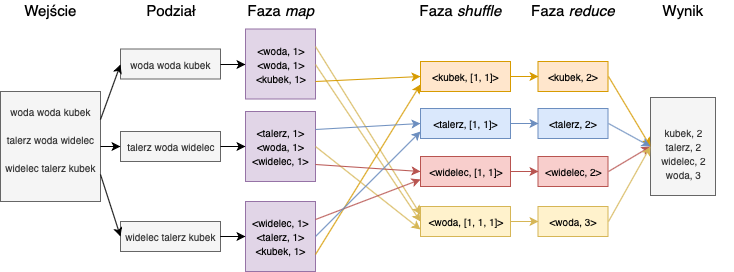
\includegraphics[width=15cm]{mapreduce_word_count.png}

Dodatkowo MapReduce dba o poprawne zarządzanie, monitorowanie i ponowne uruchamianie uszkodzonych procesów. W standardowej konfiguracji Hadoopa, MapReduce i HDFS działają na tym samym zbiorze węzłów w klastrze. Dzięki temu możliwe jest optymalne przydzielanie procesów do danych na maszynach, co skutkuje zmniejszonym przesyłem danych oraz zwiększeniem wydajności klastra.

\subsection{YARN}

YARN jest systemem zarządzającym zasobami oraz wykonywaniem się procesów na klastrze. Został dodany w późniejszej wersji Hadoopa (2.0), zastępując MapReduce w kwestii zarządzania procesami i znacząco rozszerzając zakres możliwości Hadoopa. W architekturze klastra można umieścić go pomiędzy HDFS, a serwisami odpowiedzialnymi za uruchamianie aplikacji. Zajmuje się dynamicznym przydzielaniem zasobów aplikacji, optymalizacją ich zużycia oraz uruchamianiem aplikacji.

\section{Spark}

Paragraf zostały stworzony w oparciu o \cite{zaharia2010spark}. Spark jest otwartym frameworkiem pozwalającym na szybkie i efektywne przetwarzanie dużych zbiorów danych. Motywacją do stworzenia Sparka były ograniczenia stawiane przez Hadoopa w postaci intesywnego używania dysku oraz niemożliwości wykorzystania danych pośrednich na potrzeby kolejnych operacji. W Hadoopie dane można wykorzystać dopiero po ich wcześniejszym zapisaniu do systemu plików. Spark natomiast umożliwia ponowne przetwarzanie cząstkowych danych bez konieczności ich zapisu, a następnie odczytu. Framework działa w oparciu o technologię \textit{in-memory}, umożliwiającą wykonywanie większości obliczeń w pamięci operacyjnej. W skład podstawowego rozwiązania Spark wchodzą:
\begin{itemize}
    \item SparkCore
    \item Menedżer zasobów
    \item Rozproszony system danych
    \item RDD (ang. \textit{Resilient Distributed Datasets})
\end{itemize}

Spark posiada dwa tryby przetwarzania danych: wsadowy i strumieniowy. Znajduje zastosowanie w procesach ETL, analizie danych, uczeniu maszynowym oraz algorytmach grafowych.


\subsection{SparkCore}
SparkCore jest zbiorem bibliotek wspierającym i integrującym pozostałe moduły Sparka. Tworzy warstwę abstrakcji do zarządzania systemem. Zapewnia API wysokiego poziomu dla języków: Scala, Java, Python i R.

\subsection{Menedżer zasobów}
Aplikacja Sparka to niezależne zbiory procesów nadzorowane i zarządzane przez obiekt \textit{SparkContext} tworzony w głównym procesie aplikacji. Spark nie zajmuje się zarządzaniem zasobami. W tym celu wykorzystywany jest wcześniej opisany Hadoop YARN lub podobny w działaniu Apache Mesos. Na każdym węźle klastra, aplikacji zostaje przydzielony proces wykonawczy odpowiedzialny za jej uruchamianie oraz zarządzanie danymi i zasobami.

\subsection{Rozproszony system danych}
Pomimo rozwiązania \textit{in-memory} czasem zachodzi potrzeba zapisu informacji do trwałego systemu danych. Spark wspiera szeroką gamę rozproszonych systemów przechowywania danych. Na liście znajdują się między innymi: Hadoop HDFS, Amazon S3, Cassandra czy Elasticsearch.

\subsection{Resilient Distributed Datasets}
RDD to podstawowa warstwa abstrakcji danych. Jest to kolekcja obiektów, rozproszona pomiędzy węzły klastra, umożliwiająca bezpieczne i efektywne wykonywanie operacji równoległych. Główne cechy RDD to:
\begin{itemize}
    \item odporność na błędy (ang. \textit{resilient}) - w przypadku awarii węzła klastra, Spark jest w stanie ponownie obliczyć brakujące lub zniszczone części danych. Odtwarzanie fragmentów danych jest możliwe dzięki grafom wykonania aplikacji.
    \item rozproszenie danych (ang. \textit{distributed}) - dane kolekcji są trzymane na wielu węzłach klastra jednocześnie.
    \item kolekcjonowanie danych (ang. \textit{dataset}) - RDD przechowuje obiekty wszelkiego rodzaju, począwszy od typów podstawowych, aż do złożonoych rekordów danych.
    \item zrównoleglenie - obliczenia i przekształcenia wykonywane są w sposób równoległy.
    \item \textit{in-memory} i utrwalanie danych - RDD jest traktowane jak regularny obiekt, zatem jest przechowywane w pamięci operacyjnej tak długo jak to potrzebne. Istnieje możliwość trwałego zapisu RDD do pamięci podręcznej lub zintegrowanego systemu przechowywania danych, zapewniając tym samym szybszy dostęp do danych pomiędzy procesami.
    \item leniwa ewaluacja - dane zawarte w RDD nie są dostępne i przetwarzane do momentu wywołania akcji.
    \item stałość - raz stworzone RDD nie może być zmienione, może być jedynie przekształcone w nowe RDD.
    
\end{itemize}

RDD wspierają dwa typy operacji:
\begin{itemize}
    \item \textit{przekształcenia / transformacje} - leniwie wykonywane obliczenia i operacje zwracające nowe RDD np: \textit{map}, \textit{filter}, \textit{join}
    \item \textit{akcje} - obliczenia wykonywane na RDD i zwracające wynik np: \textit{reduce}, \textit{count}
\end{itemize}

Podstawową jednostką RDD jest partycja, która jest logiczną częścią rozproszonego zbioru danych. Liczbę partycji można kontrolować. Spark optymalizuje przesył danych przez sieć, przez co stara się odtworzyć logiczny podział danych na ich fizyczne odpowiedniki.

Stworzenie RDD umożliwiło efektywne implementowanie:
\begin{itemize}
    \item interaktywnych narzędzi do analizy danych i wykonywania zapytań
    \item iteracyjnych algorytmów używanych w uczeniu maszynowym czy analizie grafów
\end{itemize}

\section{Hadoop vs Spark}

Hadoop powstał na trzy lata przed Sparkiem i przez ten czas bardzo dobrze spisywał się jako framework do przetwarzania dużych danych. MapReduce spełniał swoją funkcję jako paradygmat liniowego przetwarzania danych. Jednak z upływem czasu pojawiły się nowe potrzeby, dla których Hadoop nie mógł znaleźć zastosowania. Napisanie skomplikowanego algorytmu przy użyciu MapReduce jest czasochłonne. Dodatkowo zaimplementowane rozwiązanie jest zazwyczaj wolne z powodu wielu kroków pośrednich, z których każdy zostaje zapisany do systemu plików. W celu usprawnienia powyższych aspektów został stworzony Spark. Umożliwia on pisanie efektywnych i skomplikowanych algorytmów rozproszonych. Używanie grafów wykonań oraz technologii \textit{in-memory} znacząco zredukowało czas wykonania programów. Poniżej przedstawiono wykres porównujący rezultaty sortowania danych przy użyciu Hadoop MapReduce i Sparka. Program napisany w Sparku posortował dane 3 razy szybciej, używając 10 razy mniej maszyn.


\begin{figure}[H]
    \caption{Porównanie rekordów Hadoopa (2013) i Sparka (2014) w sortowaniu 100 TB danych używając testu wydajności \textit{Daytona Gray} \cite{Armbrust:2015:SSR:2824032.2824080}.}
    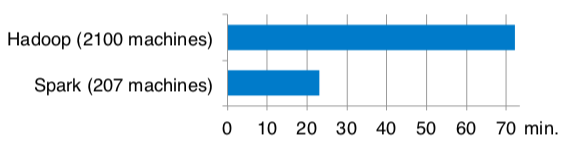
\includegraphics[width=15cm]{hadoop_vs_spark.png}
\end{figure}

Dodatkowo Spark udostępnia bardzo rozbudowane API do języków Scala, Java, Python i R. W przeciwieństwie do Hadoopa, tworzenie nowych algorytmów jest intuicyjne, łatwe i szybkie. Oba frameworki posiadają cały szereg zintegrowanych frameworków ułatwiających przetwarzanie dużych danych, jednak to Spark jest obecnie bardziej rozwijanym projektem.

\chapter{Algorytmy minimalne}\label{algorytmy_minimalne}

\section{Definicja}

Oznaczmy \textit{S} jako zbiór obiektów w rozpatrywanym problemie. Niech \textit{n} będzie liczbą obiektów wchodzących w skład \textit{S}, a \textit{t} liczbą maszyn w systemie. Zdefiniujmy \textit{m = n/t}, czyli liczbę obiektów na każdej z maszyn w przypadku równomiernego rozproszenia \textit{S}. Rozważmy algorytm rozwiązujący pewien problem na zbiorze \textit{S}. Mówimy, że algorytm jest \textit{minimalny} jeżeli posiada wszystkie z następujących własności \cite{tao2013minimal}:
\begin{itemize}
    \item \textit{ograniczona pamięć} - w każdym momencie, każda z maszyn zużywa \textit{O(m)} pamięci.
    \item \textit{ograniczony przesył danych} - w każdej rundzie MapReduce / transformacji RDD, każda z maszyn wysyła i odbiera przez sieć co najwyżej \textit{O(m)} informacji.
    \item \textit{stała liczba rund} - algorytm musi zakończyć się po stałej liczbie rund / transformacji RDD.
    \item \textit{optymalność obliczeń} - każda maszyna musi w całości wykonać \(O(T_{seq} / t\)) obliczeń, gdzie \(T_{seq}\) jest czasem potrzebnym na rozwiązanie problemu na pojedynczej maszynie sekwencyjnej. Mianowicie algorytm powinien otrzymać przyspieszenie rzędu \(t\), używając równolegle \(t\) maszyn.
\end{itemize}

Fazy i rundy MapReduce oraz transformacje RDD są wzajemnie wyrażalne. Oznacza to, że obliczenia wykonywane w paradygmacie MapReduce można wyrazić przekształceniami RDD i odwrotnie. Z tego powodu opisy przedstawionych algorytmów minimalnych zostały zapisane tylko w paradygmacie MapReduce.
\section{TeraSort}

TeraSort jest równoległym algorytmem sortującym. Na wejściu mamy dany zbiór \(S\) składający się z \(n\) porównywalnych obiektów. Do dyspozycji mamy \(t\) maszyn \(M_1, ..., M_t\). Początkowo zbiór \(S\) jest równomiernie rozproszony na maszynach. Rezultatem algorytmu jest stan, w którym obiekty na maszynie \(M_i\) są posortowane oraz poprzedzają obiekty na maszynach \(M_j\) dla każdego \(1 \leq i < j \leq t\). Parametryzowany zmienną \(\rho \in (0, 1]\) algorytm TeraSort składa się z następujących faz MapReduce \cite{tao2013minimal}: \\

\textbf{Runda 1}
\begin{itemize}
    \item \textit{Map-shuffle} \\
    Na każdej z maszyn \(M_i\) (\(1 \leq i \leq t)\), odczytujemy z pamięci lokalnej obiekty wejściowe algorytmu i każdy z nich wybieramy z prawdopodobieństwem \(\rho\). Na koniec wysyłamy wybrane elementy na wszystkie maszyny \(M_1, ..., M_t\).
    \item \textit{Reduce} \\
    Niech \(S^{\prime}\) oznacza zbiór elementów otrzymanych z fazy \(map\), a \(s = |S^{\prime}|\). Początkowo sortujemy \(S^{\prime}\), a następnie wybieramy obiekty graniczne \(b_1, ..., b_{t-1}\), gdzie \(b_i\) jest obiektem o indeksie \(i*\lceil{s / t}\rceil\) dla \(1 \leq i \leq t-1\).
\end{itemize}

\textbf{Runda 2}
\begin{itemize}
    \item \textit{Map-shuffle} \\
    Każda maszyna \(M_i\) odczytuje z pamięci lokalnej początkowe obiekty i wysyła elementy należące do przedziału \((b_{j-1}, b_j]\) na maszynę \(M_j\), dla każdego \(1 \leq j \leq t\), gdzie \(b_0 = -\infty\) oraz \(b_t = \infty\).
    \item \textit{Reduce} \\
    Każda maszyna \(M_i\) sortuje obiekty otrzymane z fazy \(map\).
\end{itemize}


\section{Lista rankingowa}

Niech \(S\) oznacza zbiór \(n\) porównywalnych obiektów wejściowych. Rezultatem algorytmu jest zwrócenie pozycji rankingowej dla każdego elementu należącego do \(S\). Problem można rozwiązać w czasie \textit{O(n log n)} na pojedynczej maszynie. Poniżej została przedstawiona wersja równoległa algorytmu w oparciu a paradygmat MapReduce \cite{tao2013minimal}. \\

\textbf{Rundy 1 - 2} \\
Sortujemy \(S\) przy użyciu algorytmu \(TeraSort\). \\

\textbf{Runda 3} \\
Niech \(Sorted_i\) oznacza posortowany zbiór obiektów na maszynie \(M_i\), dla \(1 \leq i \leq t\).
\begin{itemize}
    \item \textit{Map-shuffle} \\
    Każda maszyna \(M_i\) wysyła \(|Sorted_i|\) na maszyny \(M_{i+1}, ..., M_t\).
    \item \textit{Reduce} \\
    Niech:
    \begin{itemize}
        \item $R_i = \sum_{j \leq i-1} \ |Sorted_j|$
        \item \(localRank(o) = |\{o^\prime \in Sorted_i : \ o^\prime \leq o\}|\) dla każdego \(o \in Sorted_i\)
    \end{itemize}
    Numer rankingowy wynosi: \\
    
    $$rank(o) = R_i + localRank(o)$$
    
\end{itemize}

\section{Statystyki prefiksowe}
Niech \(S\) oznacza zbiór \(n\) porównywalnych obiektów wejściowych, a \(stat\) będzie funkcją statystyk rozdzielną na zbiorze \(S\). Z rozdzielności wynika zatem, że \(stat(S)\) może zostać obliczone w czasie stałym ze \(stat(S_1)\) i \(stat(S_2)\), gdzie \(S_1\) i \(S_2\) tworzą podział \(S\), czyli \(S_1 \cup S_2 = S\) oraz \(S_1 \cap S_2 = \emptyset\). Rezultat algorytmu definiujemy następująco \cite{tao2013minimal}:
\begin{center}
\(prefixStat(o, stat) = stat(\{o^\prime \in S: \ o^\prime < o\})\) dla każdego \(o \in S\) \\
\end{center}

\textbf{Rundy 1 - 2} \\
Sortujemy \(S\) przy użyciu algorytmu \(TeraSort\). \\

\textbf{Runda 3} \\
Niech \(Sorted_i\) oznacza posortowany zbiór obiektów na maszynie \(M_i\), dla \(1 \leq i \leq t\).
\begin{itemize}
    \item \textit{Map-shuffle} \\
    Każda maszyna \(M_i\) wysyła \(stat(Sorted_i)\) na maszyny \(M_{i+1}, ..., M_t\).
    \item \textit{Reduce} \\
    Niech
    \begin{itemize}
        \item \(V_i = stat(\{stat(Sorted_j)\})\) dla \(j \leq i-1\)
        \item \(prefixLocal(o, stat) = stat(\{o^\prime \in Sorted_i: \ o^\prime < o \})\) dla każdego \(o \in Sorted_i\)
    \end{itemize}
    Statystyki prefiksowe wynoszą: \\
    
    \centering
    \(prefixStat(o, stat) = V_i + prefixLocal(o, stat)\) dla każdego \(o \in Sorted_i\)
\end{itemize}

\section{Grupowanie}
Niech \(S\) oznacza zbiór \(n\) porównywalnych obiektów wejściowych, a \(stat\) będzie funkcją statystyk rozdzielną na zbiorze \(S\). Dodatkowo dla każdego \(o \in S\) istnieje funkcja \(key(o)\) zwracająca obiekt będący porównywalnym kluczem danego obiektu \(o\). Grupą \(G\) nazwiemy maksymalny zbiór obiektów, dla których funkcja \(key\) zwraca tą samą wartość. Rezultat algorytmu \textit{grupowania} definiujemy następująco \cite{tao2013minimal}:
\begin{center}
\(groupBy(G, stat) = stat(G)\) dla każdej grupy \(G\) na zbiorze \(S\) \\
\end{center}

\textbf{Rundy 1 - 2} \\
Sortujemy \(S\) przy użyciu algorytmu \(TeraSort\). \\

\textbf{Runda 3} \\
Niech \(Sorted_i\) oznacza posortowany zbiór obiektów na maszynie \(M_i\), dla \(1 \leq i \leq t\).

\begin{itemize}
    \item \textit{Map-shuffle} \\
    Niech:
    \begin{itemize}
        \item \(k_{min} = min(\{key(o) : \ o \in Sorted_i \})\)
        \item \(k_{max} = max(\{key(o) : \ o \in Sorted_i \})\)
    \end{itemize}
    
    Dla każdego klucza \(k \in \{key(o): \ o \in Sorted_i\}\) obliczamy grupę \(G_k\), a następnie
    dla kluczy \(k\) takich, że \(k \neq k_{min} \ oraz \ k \neq k_{max}\) wysyłamy parę \((k, stat(G_k))\) na maszynę \(M_i\).
    Dodatkowo wysyłamy \((k_{min}, stat(G_{k_{min}}))\) na maszynę \(M_1\) oraz jeżeli \(k_{min} \neq k_{max}\), to wysyłamy również \((k_{max}, stat(G_{k_{max}}))\) na maszynę \(M_1\).

    \item \textit{Reduce} \\
    Na maszynach \(M_2, ..., M_t\) mamy już gotowe wyniki grupowania. Natomiast na maszynie \(M_1\) niech \((k_1, w_1), ..., (k_x, w_x)\) oznaczają pary otrzymane z fazy \(map\), gdzie \(x \in [t, 2t]\). Dla każdej grupy, której klucz \(k\) jest wśród otrzymanych par, wynikiem algorytmu jest:\\
            $$G_k = stat(\{w_j: \ k = k_j\})$$
\end{itemize}
\section{Pół-złączenia}
Niech \(R\) i \(T\) będą dwoma zbiorami z tej samej dziedziny. Dla każdego obiektu \(o \in R \ \cup \  T\) istnieje funkcja \(key(o)\) zwracająca klucz obiektu \(o\). Problem \textit{pół-złączeń} polega na znalezieniu wszystkich obiektów \(o \in R\), takich że istnieje obiekt \(o^\prime \in T\), dla którego \(key(o) = key(o^\prime)\). Problem posiada rozwiązanie o złożoności czasowej \(O(n \ log \  n)\) na pojedynczej maszynie sekwencyjnej, gdzie \(n = |R \cup T|\) \cite{tao2013minimal}.
Niech \(S = R \cup T\). \\

\textbf{Rundy 1 - 2} \\
Sortujemy \(S\) przy użyciu algorytmu \(TeraSort\). \\

\textbf{Runda 3} \\
Zdefiniujmy \(R_i\) oraz \(T_i\) jako zbiory obiektów znajdujących się na maszynie \(M_i\) i początkowo należących odpowiednio do zbiorów \(R\), \(T\).

\begin{itemize}
    \item \textit{Map-shuffle} \\
    Na każdej maszynie \(M_i\), dla \(1 \leq i \leq t\), wysyłamy do wszystkich maszyn następujące dwie wartości:
        \begin{itemize}
            \item \(min(\{key(o): o \in T_i\})\)
            \item \(max(\{key(o): o \in T_i\})\)
        \end{itemize}
    \item \textit{Reduce} \\
    Niech \(T_{border}\) będzie zbiorem kluczy otrzymanych z fazy \(map\). Na każdej z maszyn \(M_i\), dla \(1 \leq i \leq t\), zwracamy obiekt \(o \in R_i\) jako część rezultatu, gdy
            $$key(o) \in T_i \cup T_{border}$$

\end{itemize}

\section{Sortowanie z perfekcyjnym zrównoważeniem} \label{perfect_sort}

Niech \(S\) będzie zbiorem składającym się z \(n\) porównywalnych obiektów. Rezultatem algorytmu jest stan, w którym każda z maszyn \(M_1, ..., M_{t-1}\) zawiera dokładnie \( \lceil n / t \rceil\) obiektów, a maszyna \(M_t\) zawiera pozostałe. Dodatkowo obiekty na maszynie \(M_i\), dla \(1 \leq i \leq t\), są posortowane oraz poprzedzają obiekty na maszynach \(M_j\) dla \(1 \leq i < j \leq t\). \\

Niech \(m = \lceil n / t \rceil\) oraz załóżmy, że \(m\) jest liczbą całkowitą. Jeżeli nie jest, to dokładamy do zbioru \(S\) co najwyżej \(t - 1\) nieznaczących obiektów, tak aby \(n\) było wielokrotnością \(t\). \\

\textbf{Rundy 1 - 3} \\
Na zbiorze \(S\) wykonujemy algorytm \textit{listy rankingowej}. Niech \(rank(o)\) dla \(o \in S\) oznacza pozycję rankingową obiektu \(o\). \\

\textbf{Runda 4} \\
Wykonujemy tylko fazę \textit{Map-shuffle}, w której dla każdego obiektu \(o\) na maszynie \(M_i\), dla \(1 \leq i \leq t\), wysyłamy go na maszynę \(M_j\), gdzie \(j = \lceil rank(o) / m \rceil\).

\section{Statystyka okienkowa}
Niech:
\begin{itemize}
    \item \(S\) - zbiór \(n\) porównywalnych obiektów
    \item \(l\) - wielkość okna statystyk, \(l \leq n\)
    \item \(stat\) - funkcja statystyk rozdzielna na zbiorze \(S\)
\end{itemize}

Dla każdego \(o \in S\) zdefiniujmy \(window(o)\) jako zbiór \(l\) największych obiektów nie przekraczających \(o\). Statystyka okienkowa obiektu \(o\) wynosi:
$$winStat(o) = stat(window(o))$$

Rezultatem algorytmu \textit{statystyki okienkowej} jest zwrócenie wartości \(winStat(o)\) dla każdego obiektu \(o \in S\) \cite{tao2013minimal}. \\

\textbf{Rundy 1 - 4} \\
Wykonujemy algorytm \textit{sortowania z perfekcyjnym zrównoważeniem}. W dalszej części algorytmu \(m = \lceil n / t \rceil\) oraz zakładamy, że \(m\) jest liczbą całkowitą. \\

\textbf{Runda 5}
\begin{itemize}
    \item \textit{Map-shuffle} \\
    Niech \(S_i\) oznacza zbiór elementów na maszynie \(M_i\), dla \(1 \leq i \leq t\). Do wszystkich maszyn wysyłamy \(W_i = stat(S_i)\). Następnie przesyłamy wszystkie obiekty zbioru \(S_i\) na maszynę \(M_{i+1}\), jeżeli \(l \leq m\), a w przeciwnym przypadku na maszyny o indeksach \(i + \lfloor (l - 1) / m \rfloor\) oraz \(i+1+\lfloor (l-1)/m \rfloor \).
    
    \item \textit{Reduce} \\
    Niech \(Loc_i\) oznacza zbiór obiektów znajdujących się po rundzie 4 na maszynie \(M_i\), dla \(1 \leq i \leq t\). Dla każdego \(o \in Loc_i\) obliczamy:
    \begin{itemize}
        \item \(\alpha = \lceil (rank(o) - l + 1) / m \rceil\)
        \item \(w_1 = stat(\{o^\prime : o^\prime \in Loc_\alpha \ and \ o^\prime \in window(o)\})\). Takie obiekty \(o^\prime\) zostały przysłane na maszynę \(M_i\) w fazie \textit{map-shuffle} rundy 5.
        \item $w_2 = \sum_{j=\alpha+1}^{i-1} W_j$
        \item jeżeli \(\alpha = i\), to \(w_3 = 0\), wpp \(w_3 = stat(\{o^\prime : o^\prime \in Loc_i \ and \ o^\prime \in window(o)\})\)
    \end{itemize}
    
    $$winStat(o) = stat(\{w_1, w_2, w_3\})$$
\end{itemize}

\chapter{Istniejące rozwiązania}

\section{Hadoop}

W podstawowej wersji Hadoopa na obecną chwilę nie istnieją ogólnodostępne implementacje wyżej przedstawionych algorytmów minimalnych. Standardowy Hadoop udostępnia ubogie API, a społeczność opensource-owa jest mało aktywna.   Dodatkowo generalizacja programów MapReduce jest trudna do osiągnięcia \cite{shvachko2010hadoop, white2012hadoop, taylor2010overview}.

Istnieje jednak cała gama frameworków rozbudowujących funkcjonalności Hadoopa. Jednym z nich jest Apache Hive. Jest to system umożliwiający czytanie, pisanie i zarządzanie ogromnymi zbiorami danych za pomocą SQL. Dzięki bogatemu API Hive'a jesteśmy w stanie wyrazić wszystkie powyższe algorytmy minimalne w języku SQL. Niestety framework działa optymalnie na danych tabelarycznych, co bardzo często wymaga ich wcześniejszego przetworzenia \cite{Huai:2014:MTA:2588555.2595630} .

Innym systemem wspierającym Hadoopa jest Apache Drill. Projekt, podobnie jak Apache Hive, pozwala na wykonywanie efektywnych zapytań SQL na ogromnych zbiorach danych. Z tą różnicą, że Apache Drill dobrze działa również na danych nietabelarycznych takich jak: \textit{JSON, CSV, Avro, Parquet} \cite{apache_drill}.

Widzimy, że wyrażenie przykładowych algorytmów minimalnych jest obecnie osiągalne przy użyciu dodatkowych frameworków. Nie świadczy to jednak o tym, że biblioteka jest bezużyteczna. Stwarza ona możliwości operowania na dowolnie skomplikowanych obiektach oraz jest narzędziem przyśpieszającym proces implementacji nowych algorytmów MapReduce. Dodatkowo jest zintegrowana z podstawową wersją Hadoopa, przez co jest łatwa w użyciu.

\section{Spark}

Spark, w porównaniu do Hadoopa, udostępnia bardzo bogate API. Wśród podstawowych funkcjonalności znajdziemy sortowanie, grupowanie (bez funkcji agregacji), złączenia i wiele innych. Operowanie na przetwarzanych obiektach jest bardzo intuicyjne i zwięzłe. Dodatkowo standardowa wersja Sparka posiada moduł SparkSQL do wykonywania zapytań SQL \cite{zaharia2010spark}. Z jego pomocą jesteśmy w stanie wyrazić wszystkie przykładowe algorytmy minimalne. Niestety SparkSQL działa tylko na ustrukturyzowanych rekordach \cite{Armbrust:2015:SSR:2723372.2742797}. Podobnie jak w przypadku Hadoopa, moja biblioteka działa na danych niestrukturalnych oraz rozszerza API Sparka, dzięki czemu jest wszechstronnym narzędziem do implementacji kolejnych algorytmów minimalnych.

\chapter{Biblioteka do tworzenia algorytmów minimalnych}

Z rozdziału \ref{algorytmy_minimalne} wynika jak dużo wspólnych obliczeń i funkcjonalności posiadają poszczególne algorytmy minimalne. Należą do nich między innymi sortowanie obiektów, liczenie rozłącznych statystyk na zbiorach, wysyłanie obiektów na wybrane maszyny oraz równolegle przesyłanie wielu typów obiektów. W poniższym rozdziale przedstawię implementację mojej biblioteki, napotkane problemy i ich rozwiązania. Dodatkowo porównam napisane funkcjonalności z możliwymi alternatywami oraz przedstawię obecne wsparcie Hadoopa i Sparka do implementacji powyższych modułów.

\section{Wstęp}
\textit{MinimalAlgFactory} jest klasą udostępniającą API do zaimplementowanych algorytmów minimalnych. Została napisana w języku Java 8. Jej zadaniem jest połączenie implementacji algorytmów minimalnych na platformy Hadoop i Spark. Dzięki takiemu rozwiązaniu użytkownik może jednocześnie operować na dwóch frameworkach za pomocą jednego pakietu. W skład pakietu wchodzą algorytmy:
\begin{itemize}
    \item \textit{TeraSort} - sortowanie
    \item \textit{Rank} - lista rankingowa
    \item \textit{PerfectSort} - sortowanie z perfekcyjnym równoważeniem
    \item \textit{Prefix} - statystyki prefiksowe
    \item \textit{SemiJoin} - pół-złączenia
    \item \textit{GroupBy} - grupowanie
    \item \textit{SlidingAggregation} - statystyka okienkowa
\end{itemize}

\section{Hadoop}

Biblioteka na platformę Hadoop została napisana w języku Java 8. Do zarządzania projektem został użyty Apache Maven, program automatyzujący budowę oprogramowania. Odnośnie modułów Hadoopa, rozwiązanie jest oparte o Hadoop 2.8, wspieranego rozproszonym systemem plików HDFS oraz YARN-em.

\subsection{Format danych}

Problemem, który napotykamy pisząc algorytmy na platformę Hadoop jest ilość zapisu i odczytu danych z dysku lokalnego maszyny. Podstawowa wersja Hadoopa zapisuje dane jako tekst. Jest to rozwiązanie wolne i zajmujące dużo pamięci, a przesyłanie skomplikowanych obiektów jest trudne i żmudne \cite{shvachko2010hadoop, white2012hadoop}. Alternatywą dla takiego zapisu danych są serializatory. Są to programy odpowiedzialne za tłumaczenie struktur danych i obiektów do postaci umożliwiającej zapis, odczyt i przesył, tak aby mogłby zostać odtworzone do identycznego stanu jak początkowy. Istnieje cała gama formatów serializacji danych, między innymi: JSON, XML, Protobuf, Thrift i Avro. Poniżej przedstawiam porównanie serializatorów. Testy zostały przeprowadzone na dużych obiektach, typowych dla algorytmów MapReduce \cite{avro, serialization}.

\begin{figure}[H]
    \caption{Wielkości plików po serializacji w MB}
    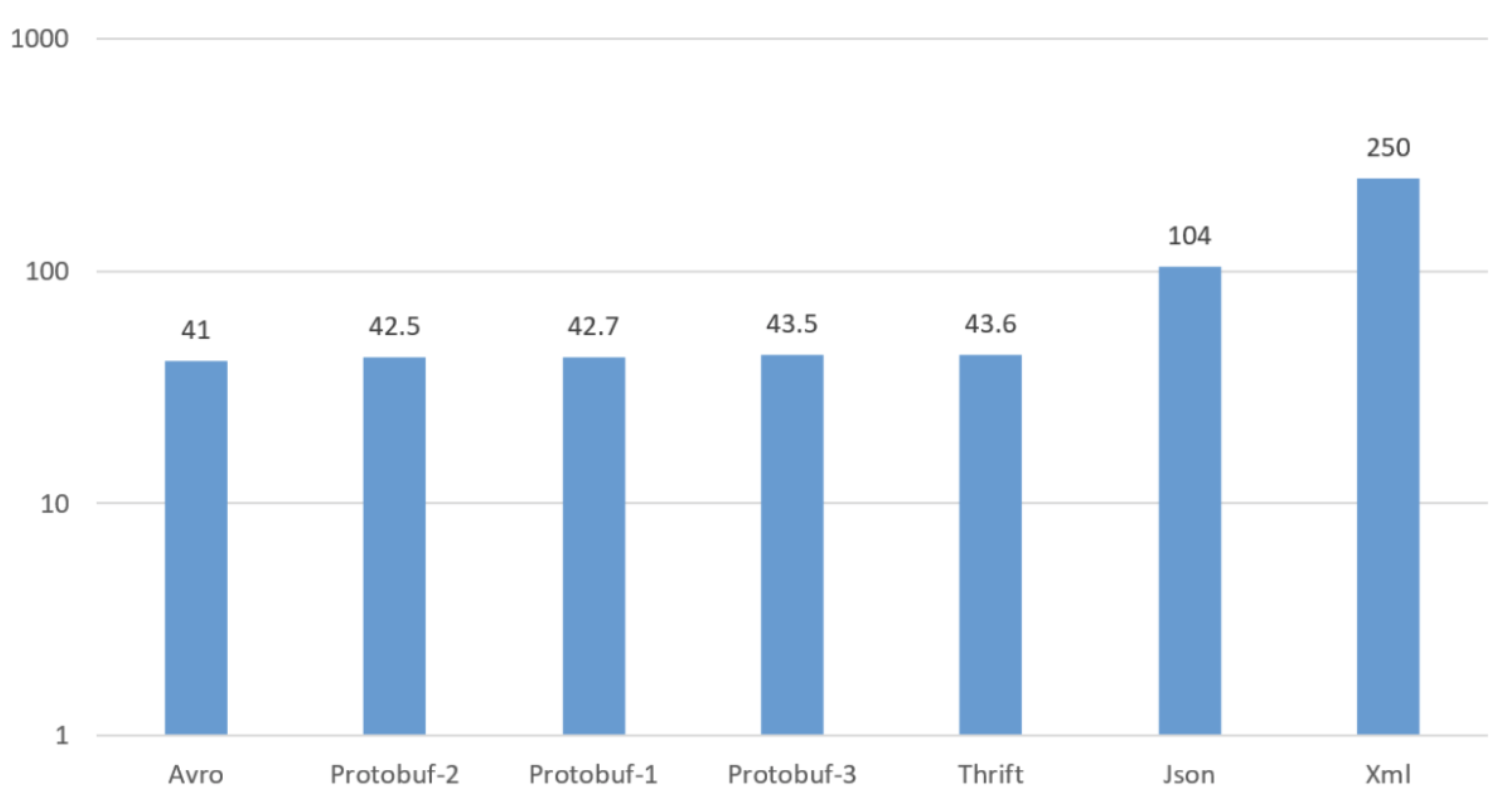
\includegraphics[width=15cm]{serialization_compression.png}
\end{figure}
\begin{figure}[H]
    \caption{Czasy serializacji i deserializacji w milisekundach}
    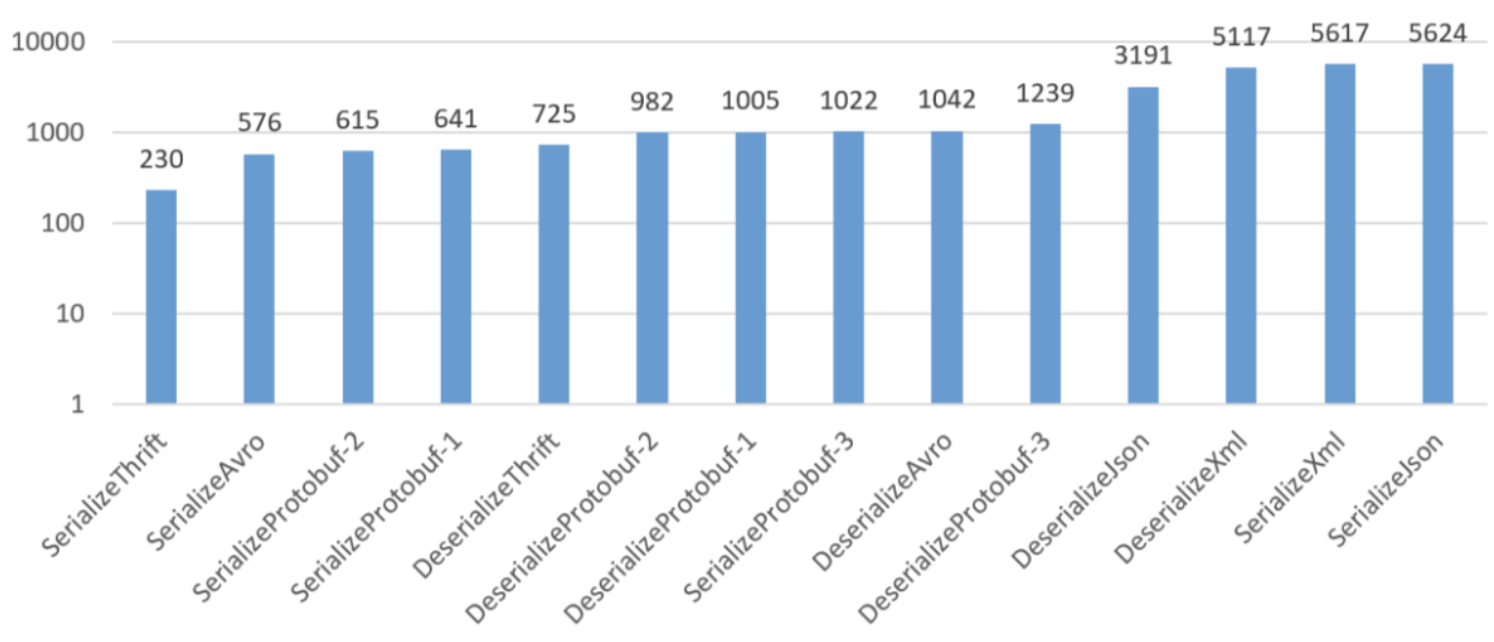
\includegraphics[width=15cm]{serialization_time.png}
\end{figure}

Z przedstawionych wykresów widać, że Avro, Protobuf i Thrift należą do czołówki serializatorów. W moim rozwiązaniu użyłem Avro, którego podstawowymi zaletami są \cite{avro}:
\begin{itemize}
    \item szybkość zapisu i odczytu
    \item kompresja danych do formatu binarnego
    \item możliwość serializowania skomplikowanych obiektów
\end{itemize}

Dodatkowo Avro ma przewagę nad Thriftem i Protobufem w obszarach takich jak \cite{avro, protobuf, thrift}:
\begin{itemize}
    \item bardzo dobra integracja z Javą i Hadoop MapReduce
    \item elastyczność schematów opisujących struktury serializowanych danych - schematy zapisu i odczytu mogą być różne
    \item możliwość mieszania kodowania binarnego i JSON
    \item klasa abstrakcyjna \textit{GenericData.Record} umożliwiająca generyczne operowanie na obiektach typu Avro
\end{itemize}

Dzięki użyciu serializatora Avro i odpowiedniej implementacji, biblioteka jest generyczna. Każda funkcja i faza MapReduce może zostać zaaplikowana do dowolnego typu danych. Jest to ogromna zaleta biblioteki, ponieważ typowe programy MapReduce są pisane pod konkretne typy danych, a zmiana danych pociąga za sobą konieczność poprawiania programu. W ramach użycia biblioteki wymagamy od użytkownika jedynie stworzenia schematu danych (plik .avsc), a następnie wykonania pojedynczej, standardowej komendy pakietu Avro Tools, tłumaczącej ten plik na klasę w Javie.

Biblioteka używa także klasy \textit{SchemaBuilder}, pozwalającej na dynamiczne budowanie schematów Avro, tym samym umożliwiając przesyłanie generycznych obiektów między fazami i rundami MapReduce.

Dzięki integracji Avro z Javą możliwe jest modyfikowanie obiektów Avro, tak aby udostępniały konkretne funkcjonalności. Stworzenie klasy abstrakcyjnej, po której dziedziczą obiekty Avro zmusza użytkownika do zaimplementowania wszystkich niezbędnych metod, a tym samym ułatwia korzystanie z biblioteki.

\subsection{Zarządzanie maszynami}

W przedstawionych algorytmach minimalnych można zauważyć jak ważna jest numeracja maszyn wchodzących w skład klastra. Niezwykle istotne jest utrzymywanie kolejności obiektów między maszynami. Dodatkowo fazy MapReduce wymagają wysyłania obiektów na konkretne maszyny. Także niektóre obliczenia wykonywane są tylko na wybranych maszynach.

Niestety Hadoop nie umożliwia ponumerowania lub oznaczania maszyn. Wszystkie maszyny oprócz \textit{NameNode} są równoważne i to YARN odpowiada za docelowe rozmieszczenie plików. Zaletą takiego rozwiązania jest fakt, że YARN wybierze maszyny, które są najbliżej danych i przesył informacji zostanie zoptymalizowany.

Rozwiązaniem, które zastosowałem jest wykorzystanie klucza, z pary wysyłanej przez MapReduce, jako numeru maszyny. Wszystkie fazy MapReduce zaimplementowane w bibliotece operują na parach \textit{<numerMaszyny, obiekty>}. Dzięki takiemu rozwiązaniu wszystkie obiekty, które powinny znaleźć się na maszynie \(M_i\), zostaną przetworzone przez jeden proces \textit{reduce}. Takie rozwiązanie pozwala symulować numerowanie maszyn w systemie oraz nie ingerować w działanie YARN-a.

Niech \(i, j \in [0, \ liczbaMaszyn]\). W ramach biblioteki zostały zaimplementowane metody umożliwiające wysyłanie obiektów na:
\begin{itemize}
    \item konkretną maszynę \(i\)
    \item wszystkie maszyny w przedziale \([i, j)\)
    \item wszystkie maszyny większe niż \(i\)
    \item wszystkie maszyny mniejsze niż \(i\)
    \item wszystkie maszyny w systemie
\end{itemize}

Funkcje zostały napisane w oparciu o klasy \textit{Mapper.Context} oraz \textit{Reducer.Context}, które są standardowym sposobem przesyłu danych w Hadoopie.

\subsection{Przesył różnych typów obiektów}

Implementując niektóre algorytmy minimalne napotykamy problem jednoczesnego przesyłania różnych typów obiektów między fazami lub rundami MapReduce. Standardowo funkcje \textit{map} i \textit{reduce} pozwalają na przesył jednego typu elementów. Nie istnieje także klasa krotek działająca na obiektach generycznych.

W tym miejscu z pomocą przychodzi serializator Avro i klasa \textit{SchemaBuilder}. Biblioteka algorytmów minimalnych implementuje klasę \textit{SendWrapper}, pozwalającą na wysyłanie zmieszanych typów danych. Na ten moment wspierana jest obsługa tylko dwóch typów obiektów. Rozszerzenie klasy na więcej typów jest jednak wykonalne i byłoby kompatybilne z obecną wersją biblioteki.

Klasa \textit{SendWrapper} opakowuje dwa obiekty Avro w jeden, tworząc schemat danych dynamicznie. Utworzony schemat posiada dwa opcjonalne pola. Gdy opakowujemy obiekt pierwszego typu, to drugie pole jest wartością \textit{null} i odwrotnie dla opakowywania elementu drugiego typu. Przesyłanie wartości \textit{null} jest niewielkim kosztem, który ponosimy za wspieranie funkcjonalności wysyłania dwóch typów obiektów. Dodatkowo biblioteka udostępnia funkcje pozwalające na filtrowanie elementów pierwszego / drugiego typu.

\begin{figure}[H]
    \caption{Przesyłanie dwóch typów obiektów}
    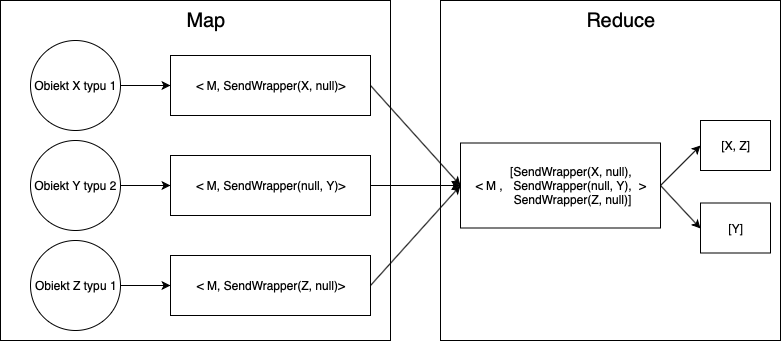
\includegraphics[width=15cm]{sending_multiple_typles.png}
\end{figure}

Alternatywą dla tego rozwiązania jest ręczne zapisywanie jednego z typów do pliku na lokalną pamięć maszyny, a następnie odczytywanie go w odpowiedniej fazie. Wadą takiego sposobu jest fakt, że rezygnujemy z automatycznego obsługiwania plików przez MapReduce. Dodatkowo jest to wolniejsze rozwiązanie, ponieważ wykonywalibyśmy dwa razy więcej operacji odczytu i zapisu.

\subsection{Statystyki}

Kolejnym zagadnieniem jest implementacja funkcji statystyk rozdzielnej na zdefiniowanym zbiorze obiektów. Rozwiązaniem, które zastosowałem jest stworzenie abstrakcyjnej klasy Avro -  \textit{StatisticsAggregator} deklarującej dwie funkcje abstrakcyjne:
\begin{enumerate}
    \item \textit{public abstract void init(GenericRecord record)} - definiuje tworzenie statystyk na podstawie obiektu. Klasa \textit{GenericRecord} jest klasą abstrakcyją obiektów Avro.
    \item \textit{public abstract StatisticsAggregator merge(StatisticsAggregator that)} - opisuje sposób łączenia dwóch statystyk, \(stat(S) = merge(stat(S_1), stat(S_2))\), gdzie \(S_1\) i \(S_2\) tworzą podział \(S\), czyli \(S_1 \cup S_2 = S\) oraz \(S_1 \cap S_2 = \emptyset\).
\end{enumerate}

Użytkownik powinien stworzyć podklasę klasy \textit{StatisticsAggregator} i napisać definicje powyższych funkcji abstrakcyjnych. Proces implementacji składa się z następujących kroków:
\begin{enumerate}
    \item Stworzenie schematu \textit{.avsc} dla klasy statystyk. Obiekty klasy statystyk są regularnymi obiektami, które są serializowalne i przesyłane między fazami MapReduce.
    \item Wygenerowanie klasy w Javie na podstawie pliku \textit{.avsc}.
    \item Zmodyfikowanie klasy utworzonej w kroku 2. Należy:
        \begin{itemize}
            \item podziedziczyć po klasie \textit{StatisticsAggregator}
            \item zaimplementować funkcje \textit{init} oraz \textit{merge}
        \end{itemize}
\end{enumerate}

Zaletami takiego podejścia są:
\begin{itemize}
    \item definiowanie dowolnie skomplikowanych funkcji statystyk
    \item wykonywanie jednocześnie kilku funkcji statystyk
    \item przechowywanie dodatkowych informacji związanych ze statystykami
\end{itemize}

Biblioteka udostępnia także funkcje agregujące statystyki takie jak:
\begin{itemize}
    \item \textit{scanLeft} - statystyki prefiksowe
    \item \textit{foldLeft} - agregacja statystyk z listy do pojedynczej wartości
\end{itemize}

Dodatkowo została stworzona klasa \textit{RangeTree} umożliwiająca liczenie statystyk na przedziałach, w sposób sekwencyjny na pojedynczej maszynie. \textit{RangeTree} jest w pełni serializowalne co pozwala na przesyłanie uszeregowanych statystyk, a następnie wykonywanie optymalnych zapytań. Klasa implementuje klasyczne, pełne drzewo binarne oraz funkcje:
\begin{itemize}
    \item \textit{public void insert(StatisticsAggregator element, int pos)} - wrzucanie statystyk do drzewa
    \item \textit{public StatisticsAggregator query(int start, int end)} - agregacja statystyk z zakresu \([start, end)\)
\end{itemize}

\subsection{Użytkowanie}

Pisanie programów na platformę Hadoop wymaga wiedzy i dokładności. Standardowo na wstępie użytkownik ustawia w konfiguracji programu wszelkie niezbędne parametry. Jednak system nie sprawdzana ich obecności i poprawności. Brak jednego z nich skutkuje zatrzymaniem wykonania programu i czasem straconym na znalezienie brakujących zmiennych.

W bibliotece algorytmów minimalnych wymagamy od użytkownika uzupełnienia wszystkich niezbędnych parametrów, a brak któregoś z nich jest sygnalizowany czytelnym komunikatem. Dodatkowo sprawdzana jest ich poprawność, aby uchronić użytkownika od banalnych błędów.

Biblioteka udostępnia także API do zarządzania plikami Avro na pamięci lokalnej maszyny. W jego skład wchodzą funkcje takie jak: \textit{zapis}, \textit{odczyt}, \textit{usuwanie}, ale także \textit{łączenie} dwóch plików Avro.

Dodatkowo istnieje funkcja, operująca na konfiguracji programu, zapisująca i odczytująca komparator obiektów Avro. Dzięki tej metodzie użytkownik raz zapisuje komparator do konfiguracji, a następnie może z niego korzystać w dowolnej fazie MapReduce.

\section{Spark}

Biblioteka do Sparka jest oparta o wersję Spark 2.3 i jest napisana w języku Scala 2.11. Do zarządzania projektem został użyty Apache Maven, program automatyzujący budowę oprogramowania.

\subsection{Format danych}
Format przechowywania i przesyłania danych odgrywa bardzo ważną rolę w aplikacjach rozproszonych. W przypadku Sparka nie istnieje problem zapisu obiektów jako tekst. Standardowa wersja frameworku udostępnia dwie biblioteki do serializacji \cite{karau2015learning}:
\begin{enumerate}
    \item \textit{Java serialization}
    \item \textit{Kryo serialization}
\end{enumerate}

Pierwsza biblioteka jest domyślnym sposobem serializacji obiektów w Sparku. Działa dla każdego obiektu Java, który implementuje klasę \textit{java.io.Serializable}. Niestety w przypadku serializacji dużych i skomplikowanych obiektów jest wolna. Druga biblioteka jest dużo szybsza (nawet 10 razy \cite{spark_serialization}) jednak nie wspiera wszystkich typów \textit{Serializable} i wymaga rejestrowania schematu klasy. Kryo jest rekomendowanym sposobem na zoptymalizowanie programu w Sparku. Wybór serializatora zależy od użytkownika i jest bardzo prosty do ustawienia.

\subsection{Zarządzanie maszynami}

W Sparku nie możemy operować bezpośrednio na maszynach. Przykrywa je bowiem warstwa abstrakcji w postaci kolekcji rozproszonych danych, czyli RDD. Podstawową jednostką RDD są partycje. W moim rozwiązaniu to właśnie partycje symulują maszyny przedstawiane w algorytmach minimalnych.

RDD w API Sparka jest reprezentowane jako kolekcja partycji. Z tego wynika, że kolejne partycje mogą odpowiadać kolejnym maszynom. Trzeba jednak pamiętać o tym, że porządek obiektów na partycji może ulec zmianie. RDD są stałe, czyli raz stworzone nie mogą ulec zmianie. Jednak nowe RDD są tworzone przez transformacje istniejących. Przekształcenia takie jak:
\begin{itemize}
    \item \textit{map} - aplikowanie funkcji do obiektów na RDD
    \item \textit{filter} - filtrowanie obiektów RDD
    \item \textit{mapPartitions} - aplikowanie funkcji do całych partycji
\end{itemize}
 
 utrzymują porządek na partycji. Natomiast istnieją też transformacje zaburzające kolejność elementów. Należą do nich między innymi:
 \begin{itemize}
     \item \textit{sortBy} - sortowanie elementów
     \item \textit{partitionBy} - podział RDD na nowe partycje za pomocą zdefiniowanej klasy podziału
 \end{itemize}

Wysyłanie obiektów na wybrane maszyny polega na zapisaniu ich na docelowej partycji. Nie możemy jednak przesyłać pojedynczych elementów. Wszystkie operacje muszą być wykonywane na RDD. Rozwiązanie, które zaimplementowałem opiera się na przetasowywaniu RDD, a następnie jego podziale na partycje za pomocą zdefiniowanych podklas klasy \textit{Partitioner}. Niestety powyższe rozwiązanie nie gwarantuje zachowania kolejności elementów. Biblioteka algorytmów minimalnych zawiera dwie podklasy:
\begin{enumerate}
    \item \textit{KeyPartitioner} - podział RDD wyznacza klucz obiektu, który jest docelowym indeksem maszyny
    \item \textit{PerfectPartitioner} - na podstawie rankingu obiektów dzieli RDD na partycje o równym rozmiarze, zgodnie z opisem w sekcji \ref{perfect_sort}
\end{enumerate}

W przypadku wysyłania obiektów na wszystkie maszyny, została zaimplementowana też druga, konkurencyjna metoda. Wykorzystuje ona klasę \textit{Broadcast}. Polega na natychmiastowym stworzeniu stałej zapisanej w pamięci podręcznej każdego węzła klastra. Spark optymalizuje wysyłanie takich zmiennych, zatem jest to dobra opcja do przesłania kopii dużych zbiorów danych potrzebnych na wielu etapach obliczeń. W sytuacji, gdy kopie wszystkich elementów są potrzebne tylko w następnej transformacji, lepiej użyć leniwie wykonującego się \textit{Partitionera} z pierwszego rozwiązania \cite{spark_documentation}.

Tak jak w przypadku Hadoopa, udostępnione zostały następujące funkcje przesyłu obiektów na:
\begin{itemize}
    \item konkretną maszynę \(i\)
    \item wszystkie maszyny w przedziale \([i, j)\)
    \item wszystkie maszyny większe niż \(i\)
    \item wszystkie maszyny mniejsze niż \(i\)
    \item wszystkie maszyny w systemie
\end{itemize}

gdzie \(i, j \in [0, \ liczbaMaszyn]\).

\subsection{Przesył różnych typów obiektów}

Na platformie Spark również doświadczamy problemu przesyłania różnych typów obiektów między transformacjami RDD. W tej sekcji przedstawię możliwe rozwiązania tego problemu oraz uargumentuję wybór zaimplementowanej metody.

Pierwszym ze sposobów jest użycie klasy \textit{Broadcast}. Jak już wspomniałem wcześniej, jest to dobre rozwiązanie, gdy chcemy używać przesyłanych obiektów na wszystkich maszynach i w dodatku w kilku transformacjach. W przeciwnym przypadku marnujemy tylko zasoby Sparka.

Inną możliwością jest wykorzystanie klasy \textit{Accumulator} udostępnianej przez Sparka. Obiekty tej klasy są współdzielonymi akumulatorami, do których można dodawać obiekty tylko podczas przemiennej, asocjacyjnej transformacji np: \textit{map}. Co więcej, węzły wykonawcze (\textit{DataNode}) mogą tylko zapisywać dane, a jedynie węzeł główny (\textit{NameNode}) może je odczytywać \cite{spark_documentation}. Niestety oba powyższe fakt znacząco ograniczają możliwości użycia akumulatorów.

Kolejnym rozwiązaniem jest zapisywanie obiektów do rozproszonego systemu danych np: HDFS. Jednak w Sparku byłoby to ogromne spowolnienie dla całego programu. Standardowo zapis danych do pamięci następuje tylko w momencie utrwalenia ostatecznych rezultatów lub gdy brakuje pamięci operacyjnej \cite{zaharia2010spark}.

Następnym sposobem jest rozwiązanie podobne do zaimplementowanego w bibliotece algorytmów minimalnych na Hadoopa. Sprowadza się ono do mieszania obiektów różnych typów na jednym RDD. Rozwiązanie wykorzystywałoby API Sparka, dzięki czemu byłoby łatwe w obsłudze i bardziej efektywne niż zapis do rozproszonego systemu danych. Niestety w momencie transformacji wymagałoby rozdzielenia obiektów, co generowałoby dodatkowe koszty czasowe.

Ostatnim i wybranym rozwiązaniem jest łączenie RDD. API Sparka udostępnia metodę \textit{zipPartitions} pozwalającą na równoległe iterowanie po od dwóch do czterech RDD, zachowując przy tym kolejność partycji i obiektów. Zaimplementowanie przesyłu różnych typów obiektów składa się z następujących kroków:
\begin{enumerate}
    \item Wysyłamy obiekty typu \textbf{I} na wybrane maszyny $\rightarrow$ powstaje nowe RDD - \textit{Rdd1}
    \item Wysyłamy obiekty typu \textbf{II} na wybrane maszyny $\rightarrow$ powstaje nowe RDD - \textit{Rdd2}
    \item Łączymy \textit{Rdd1} z \textit{Rdd2} i aplikujemy transformację:
    $$Rdd1.zipPartitions(Rdd2)\{(partitions1Iter, \ partitions2Iter) => \{ ... \}\}$$
\end{enumerate}

Jest to najbardziej efektywne i zwięzłe rozwiązanie, dodatkowo zachowujące kolejność obiektów. 

\subsection{Statystyki}

Problem liczenia statystyk na Sparku rozwiązałem w sposób bardzo podobny do tego na Hadoopie. Została stworzona klasa abstrakcyjna \textit{StatisticsAggregator} deklarująca funkcję abstrakcyjną
$$def \ merge(statisticsAggregator: S): S $$ gdzie \textit{S} jest podklasą klasy \textit{StatisticsAggregator}. Funkcja \textit{merge}, tak samo jak w Hadoopie, definuje proces łączenia dwóch statystyk. Po stronie użytkownika pozostaje stworzenie klasy \textit{S} oraz zdefiniowanie funkcji $init: T \rightarrow S$, gdzie \textit{T} jest typem obiektów wejściowych. Definiowanie funkcji \textit{init} poza klasą \textit{S} umożliwia większą elastyczość i generalizację w użytkowaniu i pisaniu algorytmów.

Biblioteka algorytmów minimalnych udostępnia także następujące operacje na statystykach:
\begin{itemize}
    \item \textit{scanLeft} - statystyki prefiksowe dla kolekcji
    \item \textit{foldLeft} - agregacja statystyk z kolekcji do pojedynczej wartości
    \item \textit{scanLeftPartitions} - statystyki prefiksowe na partycjach zawartych w RDD
    \item \textit{partitionStatistics} - statystyki dla każdej partycji zawartej w RDD
\end{itemize}

Identycznie jak w rozwiązaniu na Hadoopa, została zaimplementowana klasa \textit{RangeTree}, udostępniające takie samo API.

\subsection{Użytkowanie}

Pisanie programów w Sparku jest łatwe i intuicyjne. Takie założenia spełnia też biblioteka algorytmów minimalnych. Punktem wejściowym jest podanie dwóch argumentów:
\begin{itemize}
    \item \textit{SparkSession} - obiekt niezbędny do uruchomienia każdego programu w Sparku
    \item \textit{numberOfPartitions} - liczba maszyn (partycji)
\end{itemize}

W przypadku uruchamiania algorytmów nieuwzględniających liczenia statystyk, takich jak: \textit{TeraSort}, \textit{ranking}, \textit{pół-złączenia} użytkownik musi zdefiniować komparator obiektów wejściowych. Komparator jest pojedynczą funkcją, co pozwala na używanie wielu z nich przy raz wczytanych danych.

Natomiast algorytmy agregujące statystyki, czyli: \textit{statystyki prefiksowe}, \textit{grupowanie}, \textit{statystyki okienkowe} wymuszają dodatkowe zaimplementowanie podklasy \textit{StatisticsAggregator} oraz zdefiniowanie funkcji \textit{init}, tak jak zostało to opisane w poprzednim paragrafie.

\chapter{Zalety biblioteki}

Pierwszą z zalet biblioteki algorytmów minimalnych jest redukcja pisanego kodu. W przypadku Sparka jest niewielka, ze względu na zwięzłość samego frameworka i bogatego API, jednak w Hadoopie jest bardzo widoczna. Głównie przyczyniają się do tego generalizacja faz MapReduce oraz serializowalny format danych. Sama tylko możliwość posortowania dowolnych obiektów ma ogromne znaczenie w redukcji kodu. Używając zaimplementowanej metody \textit{TeraSort} użytkownik oszczędza około 200 linii kodu. Dodatkowo wszystkie fazy MapReduce i funkcje udostępniane przez API są generyczne. Wystarczy zdefiniować klasę obiektów, a reszta implementacji pozostaje stała. Zarówno w Sparku jak i w Hadoopie, do porównywania obiektów używane są komparatory, dzięki czemu użytkownik jeszcze mniejszym nakładem czasu i pracy może testować różne wersje algorytmu.

Kolejnym ważnym aspektem jest działanie biblioteki na dowolnie skomplikowanych danych. W przypadku Sparka, użytkownik w ogóle nie musi wstępnie przetwarzać danych, natomiast w Hadoopie musi zdefiniować strukturę Avro, a następnie wygenerować klasę Javy. Jest to przewaga nad istniejącymi rozwiązaniami takimi jak Apache Hive czy SparkSQL.

Następną zaletą jest możliwość definiowania własnej funkcji statystyk. Zewnętrzne frameworki udostępniają zazwyczaj opcje agregowania wartości numerycznych lub tekstowych. Natomiast przy użyciu rozwiązania biblioteki algorytmów minimalnych, pamiętając o zachowaniu własności rozdzielności, jesteśmy w stanie implementować statystyki operujące na dowolnych obiektach.

Biblioteka udostępnia także szereg przydatnych funkcji, dzięki którym pisanie nowych algorytmów powinno być bardziej intuicyjne i efektywne.

Na koniec nie zapominajmy o własnościach algorytmów minimalnych. Wszystkie zaimplementowane algorytmy oraz funkcje API spełniają wcześniej zdefiniowane kryteria minimalności. Dzięki temu biblioteka umożliwia skuteczne przetwarzanie dużych zbiorów danych.

\chapter{Testy}

Biblioteka algorytmów minimalnych zawiera zestaw testów poprawnościowych sprawdzających działanie kodu w spreparowanym środowisku oraz skrypty testujące algorytmy minimalne w warunkach produkcyjnych. Dodatkowo w ramach pracy przeprowadziłem testy wydajnościowe. Przy użyciu generatora losowych danych typu \textit{avro} (https://github.com/confluentinc/avro-random-generator) stworzyłem dwie grupy danych ważące 1 GB (10 000 000 obiektów) i 5 GB (45 000 000 obiektów). Obiekty zostały stworzone przy pomocy następującego schematu:

\begin{lstlisting}[language=json,firstnumber=1]
{ "type": "record",
  "name": "Complex",
  "namespace": "complex.type",
  "fields":
    [
      { "name": "null_prim", "type": ["null", "int"] },
      { "name": "boolean_prim", "type": "boolean" },
      { "name": "int_prim", "type": {
          "type": "int",
          "arg.properties": {
            "range": {
              "min": -10,
              "max": 10
            }
          }
        }
      },
      { "name": "long_prim", "type": "long" },
      { "name": "float_prim", "type": "float" },
      { "name": "double_prim", "type": "double" },
      { "name": "string_prim", "type": "string" },
      { "name": "bytes_prim", "type": "bytes" },
      { "name": "middle", "type":
        { "type": "record",
          "name": "MiddleNested",
          "fields": [
            { "name": "middle_array",
              "type": {
                "type": "array",
                "items": "float"
              }
            },
            { "name": "inner",
              "type": {
                "type": "record",
                "name": "InnerNested",
                "fields": [
                  { "name": "inner_int",
                    "type": "int"
                  },
                  { "name": "inner_string",
                    "type": "string"
                  }
                ]
              }
            }
          ]
        }
      }
    ]
}
\end{lstlisting}

Testy zostały przeprowadzone na dwóch typach klastrów składających się z:
\begin{itemize}
    \item 1 NameNode + 5 DataNode
    \item 1 NameNode + 10 DataNode
\end{itemize}

Klastry zostały utworzone na platformie \textit{Amazon Web Services}. Każdy NameNode i DataNode posiadał 4-rdzeniowy procesor oraz 6 GB pamięci RAM.

Do porównywania obiektów został wykorzystany następujący komparator:
\\
\\
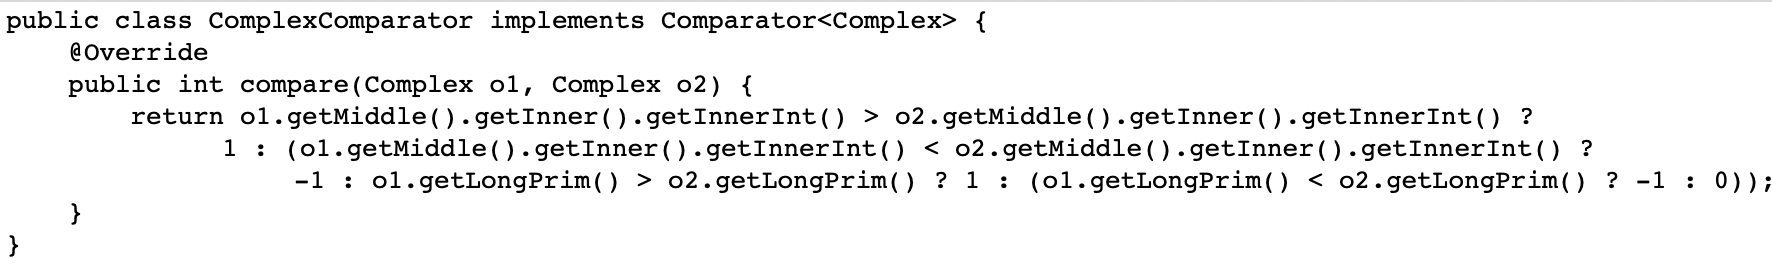
\includegraphics[width=15cm]{complex_cmp.png}

\section{Hadoop}

W poniższych sekcjach zostały przedstawione wyniki testów poszczególnych algorytmów minimalnych wykonanych na Hadoopie. Kolumny mają następujące znaczenie:
\begin{itemize}
    \item Runda - runda algorytmu MapReduce opisana w sekcji \ref{algorytmy_minimalne}
    \item Czas (s) - całkowity czas wykonania algorytmu
    \item Max zużycie pamięci (GB) - maksymalne zużycie pamięci na całym klastrze podczas wykonywania algorytmu
    \item Max przesył danych (GB) - maksymalny przesył danych wewnątrz całego klastra podczas wykonywania algorytmu
\end{itemize}

\subsection{TeraSort}

\begin{table}[H]
\centering
\caption{Wykonanie algorytmu \textit{TeraSort} na 1 GB danych przy użyciu 5 maszyn.}
\label{tab:my-table}
\resizebox{\textwidth}{!}{%
\begin{tabular}{@{}|c|c|c|c|@{}}
\toprule
\textbf{Runda} & \textbf{Czas (s)} & \textbf{Max zużycie pamięci (GB)} & \textbf{Max przesył danych (GB)} \\ \midrule
Sampling      & 43                & 4,785                            & 0,003                                    \\ \midrule
Sorting       & 104               & 12,062                           & 1,187                                    \\ \bottomrule
\end{tabular}%
}
\end{table}

\begin{table}[H]
\centering
\caption{Wykonanie algorytmu \textit{TeraSort} na 5 GB danych przy użyciu 5 maszyn.}
\label{tab:my-table}
\resizebox{\textwidth}{!}{%
\begin{tabular}{@{}|c|c|c|c|@{}}
\toprule
\textbf{Runda} & \textbf{Czas (s)} & \textbf{Max zużycie pamięci (GB)} & \textbf{Max przesył danych (GB)} \\ \midrule
Sampling      & 83                & 20,252                           & 0,005                                    \\ \midrule
Sorting       & 273               & 34,677                           & 5,099                                    \\ \bottomrule
\end{tabular}%
}
\end{table}

\begin{table}[H]
\centering
\caption{Wykonanie algorytmu \textit{TeraSort} na 1 GB danych przy użyciu 10 maszyn.}
\label{tab:my-table}
\resizebox{\textwidth}{!}{%
\begin{tabular}{@{}|c|c|c|c|@{}}
\toprule
\textbf{Runda} & \textbf{Czas (s)} & \textbf{Max zużycie pamięci (GB)} & \textbf{Max przesył danych (GB)} \\ \midrule
Sampling      & 41                & 4,643                            & 0,003                                    \\ \midrule
Sorting       & 70                & 12,303                           & 1,133                                    \\ \bottomrule
\end{tabular}%
}
\end{table}

\begin{table}[H]
\centering
\caption{Wykonanie algorytmu \textit{TeraSort} na 5 GB danych przy użyciu 10 maszyn.}
\label{tab:my-table}
\resizebox{\textwidth}{!}{%
\begin{tabular}{@{}|c|c|c|c|@{}}
\toprule
\textbf{Runda} & \textbf{Czas (s)} & \textbf{Max zużycie pamięci (GB)} & \textbf{Max przesył danych (GB)} \\ \midrule
Sampling      & 55                & 19,612                           & 0,012                                    \\ \midrule
Sorting       & 139               & 40,187                           & 5,101                                    \\ \bottomrule
\end{tabular}%
}
\end{table}

\subsection{Lista rankingowa}

\begin{table}[H]
\centering
\caption{Wykonanie algorytmu \textit{lista rankingowa} na 1 GB danych przy użyciu 5 maszyn.}
\label{tab:my-table}
\resizebox{\textwidth}{!}{%
\begin{tabular}{@{}|c|c|c|c|@{}}
\toprule
\textbf{Runda} & \textbf{Czas (s)} & \textbf{Max zużycie pamięci (GB)} & \textbf{Max przesył danych (GB)} \\ \midrule
Sampling      & 43                & 4,575                            & 0,003                                    \\ \midrule
Sorting       & 101               & 11,011                           & 1,137                                    \\ \midrule
Ranking       & 77                & 13,197                           & 1,094                                    \\ \bottomrule
\end{tabular}%
}
\end{table}

\begin{table}[H]
\centering
\caption{Wykonanie algorytmu \textit{lista rankingowa} na 5 GB danych przy użyciu 5 maszyn.}
\label{tab:my-table}
\resizebox{\textwidth}{!}{%
\begin{tabular}{@{}|c|c|c|c|@{}}
\toprule
\textbf{Runda} & \textbf{Czas (s)} & \textbf{Max zużycie pamięci (GB)} & \textbf{Max przesył danych (GB)} \\ \midrule
Sampling      & 81                & 20,452                           & 0,005                                    \\ \midrule
Sorting       & 267               & 34,687                           & 5,109                                    \\ \midrule
Ranking       & 226               & 36,123                           & 4,923                                    \\ \bottomrule
\end{tabular}%
}
\end{table}

\begin{table}[H]
\centering
\caption{Wykonanie algorytmu \textit{lista rankingowa} na 1 GB danych przy użyciu 10 maszyn.}
\label{tab:my-table}
\resizebox{\textwidth}{!}{%
\begin{tabular}{@{}|c|c|c|c|@{}}
\toprule
\textbf{Runda} & \textbf{Czas (s)} & \textbf{Max zużycie pamięci (GB)} & \textbf{Max przesył danych (GB)} \\ \midrule
Sampling      & 40                & 4,653                            & 0,003                                    \\ \midrule
Sorting       & 71                & 12,203                           & 1,123                                    \\ \midrule
Ranking       & 66                & 15,865                           & 1,094                                    \\ \bottomrule
\end{tabular}%
}
\end{table}

\begin{table}[H]
\centering
\caption{Wykonanie algorytmu \textit{lista rankingowa} na 5 GB danych przy użyciu 10 maszyn.}
\label{tab:my-table}
\resizebox{\textwidth}{!}{%
\begin{tabular}{@{}|c|c|c|c|@{}}
\toprule
\textbf{Runda} & \textbf{Czas (s)} & \textbf{Max zużycie pamięci (GB)} & \textbf{Max przesył danych (GB)} \\ \midrule
Sampling      & 53                & 19,312                           & 0,012                                    \\ \midrule
Sorting       & 138               & 39,587                           & 5,081                                    \\ \midrule
Ranking       & 120               & 38,440                           & 4,923                                    \\ \bottomrule
\end{tabular}%
}
\end{table}

\subsection{Statystyki prefiksowe}

Algorytm statystyk prefiksowych wykorzystywał sumę jako funkcję statystyk.

\begin{table}[H]
\centering
\caption{Wykonanie algorytmu \textit{statystyki prefiksowe} na 1 GB danych przy użyciu 5 maszyn.}
\label{tab:my-table}
\resizebox{\textwidth}{!}{%
\begin{tabular}{@{}|c|c|c|c|@{}}
\toprule
\textbf{Runda} & \textbf{Czas (s)} & \textbf{Max zużycie pamięci (GB)} & \textbf{Max przesył danych (GB)} \\ \midrule
Sampling      & 41                & 4,575                            & 0,003                                    \\ \midrule
Sorting       & 102               & 11,021                           & 1,137                                    \\ \midrule
Prefix        & 95                & 13,326                           & 1,148                                    \\ \bottomrule
\end{tabular}%
}
\end{table}

\begin{table}[H]
\centering
\caption{Wykonanie algorytmu \textit{statystyki prefiksowe} na 5 GB danych przy użyciu 5 maszyn.}
\label{tab:my-table}
\resizebox{\textwidth}{!}{%
\begin{tabular}{@{}|c|c|c|c|@{}}
\toprule
\textbf{Runda} & \textbf{Czas (s)} & \textbf{Max zużycie pamięci (GB)} & \textbf{Max przesył danych (GB)} \\ \midrule
Sampling      & 80                & 20,552                           & 0,005                                    \\ \midrule
Sorting       & 266               & 34,667                           & 5,106                                    \\ \midrule
Prefix        & 255               & 32,260                           & 5,185                                    \\ \bottomrule
\end{tabular}%
}
\end{table}

\begin{table}[H]
\centering
\caption{Wykonanie algorytmu \textit{statystyki prefiksowe} na 1 GB danych przy użyciu 10 maszyn.}
\label{tab:my-table}
\resizebox{\textwidth}{!}{%
\begin{tabular}{@{}|c|c|c|c|@{}}
\toprule
\textbf{Runda} & \textbf{Czas (s)} & \textbf{Max zużycie pamięci (GB)} & \textbf{Max przesył danych (GB)} \\ \midrule
Sampling      & 41                & 4,643                            & 0,003                                    \\ \midrule
Sorting       & 70                & 12,213                           & 1,133                                    \\ \midrule
Prefix        & 85                & 16,017                           & 1,148                                    \\ \bottomrule
\end{tabular}%
}
\end{table}

\begin{table}[H]
\centering
\caption{Wykonanie algorytmu \textit{statystyki prefiksowe} na 5 GB danych przy użyciu 10 maszyn.}
\label{tab:my-table}
\resizebox{\textwidth}{!}{%
\begin{tabular}{@{}|c|c|c|c|@{}}
\toprule
\textbf{Runda} & \textbf{Czas (s)} & \textbf{Max zużycie pamięci (GB)} & \textbf{Max przesył danych (GB)} \\ \midrule
Sampling      & 53                & 19,312                           & 0,012                                    \\ \midrule
Sorting       & 138               & 39,587                           & 5,081                                    \\ \midrule
Prefix        & 140               & 42,469                           & 5,185                                    \\ \bottomrule
\end{tabular}%
}
\end{table}

\subsection{Grupowanie}

Algorytm grupowania wykorzystywał sumę jako funkcję statystyk.

\begin{table}[H]
\centering
\caption{Wykonanie algorytmu \textit{grupowania} na 1 GB danych przy użyciu 5 maszyn.}
\label{tab:my-table}
\resizebox{\textwidth}{!}{%
\begin{tabular}{@{}|c|c|c|c|@{}}
\toprule
\textbf{Runda} & \textbf{Czas (s)} & \textbf{Max zużycie pamięci (GB)} & \textbf{Max przesył danych (GB)} \\ \midrule
Sampling      & 41                & 4,555                            & 0,003                                    \\ \midrule
Sorting       & 101               & 11,011                           & 1,117                                    \\ \midrule
GroupBy       & 49                & 8,899                            & 0,0001                                   \\ \bottomrule
\end{tabular}%
}
\end{table}

\begin{table}[H]
\centering
\caption{Wykonanie algorytmu  \textit{grupowania} na 5 GB danych przy użyciu 5 maszyn.}
\label{tab:my-table}
\resizebox{\textwidth}{!}{%
\begin{tabular}{@{}|c|c|c|c|@{}}
\toprule
\textbf{Runda} & \textbf{Czas (s)} & \textbf{Max zużycie pamięci (GB)} & \textbf{Max przesył danych (GB)} \\ \midrule
Sampling      & 79                & 20,532                           & 0,005                                    \\ \midrule
Sorting       & 265               & 34,657                           & 5,101                                    \\ \midrule
GroupBy       & 126               & 27,279                           & 0,0006                                   \\ \bottomrule
\end{tabular}%
}
\end{table}

\begin{table}[H]
\centering
\caption{Wykonanie algorytmu  \textit{grupowania} na 1 GB danych przy użyciu 10 maszyn.}
\label{tab:my-table}
\resizebox{\textwidth}{!}{%
\begin{tabular}{@{}|c|c|c|c|@{}}
\toprule
\textbf{Runda} & \textbf{Czas (s)} & \textbf{Max zużycie pamięci (GB)} & \textbf{Max przesył danych (GB)} \\ \midrule
Sampling      & 40                & 4,623                            & 0,003                                    \\ \midrule
Sorting       & 71                & 12,211                           & 1,113                                    \\ \midrule
GroupBy       & 51                & 10,842                           & 0,0001                                   \\ \bottomrule
\end{tabular}%
}
\end{table}

\begin{table}[H]
\centering
\caption{Wykonanie algorytmu  \textit{grupowania} na 5 GB danych przy użyciu 10 maszyn.}
\label{tab:my-table}
\resizebox{\textwidth}{!}{%
\begin{tabular}{@{}|c|c|c|c|@{}}
\toprule
\textbf{Runda} & \textbf{Czas (s)} & \textbf{Max zużycie pamięci (GB)} & \textbf{Max przesył danych (GB)} \\ \midrule
Sampling      & 52                & 19,311                           & 0,011                                    \\ \midrule
Sorting       & 137               & 39,567                           & 5,071                                    \\ \midrule
GroupBy       & 80                & 30,526                           & 0,0001                                   \\ \bottomrule
\end{tabular}%
}
\end{table}

\subsection{Statystyka okienkowa}

Algorytm statystyki okienkowej wykorzystywał sumę jako funkcję statystyk.

\begin{table}[H]
\centering
\caption{Wykonanie algorytmu \textit{statystyki okienkowej} na 1 GB danych przy użyciu 5 maszyn.}
\label{tab:my-table}
\resizebox{\textwidth}{!}{%
\begin{tabular}{@{}|c|c|c|c|@{}}
\toprule
\textbf{Runda}      & \textbf{Czas (s)} & \textbf{Max zużycie pamięci (GB)} & \textbf{Max przesył danych (GB)} \\ \midrule
Sampling           & 40                & 4,556                            & 0,003                                    \\ \midrule
Sorting            & 102               & 11,012                           & 1,116                                    \\ \midrule
Ranking            & 86                & 13,198                           & 1,093                                    \\ \midrule
PerfectSort        & 94                & 13,994                           & 1,168                                    \\ \midrule
SlidingAggregation & 141               & 16,168                           & 2,366                                    \\ \bottomrule
\end{tabular}%
}
\end{table}

\begin{table}[H]
\centering
\caption{Wykonanie algorytmu \textit{statystyki okienkowej} na 5 GB danych przy użyciu 5 maszyn.}
\label{tab:my-table}
\resizebox{\textwidth}{!}{%
\begin{tabular}{@{}|c|c|c|c|@{}}
\toprule
\textbf{Runda}      & \textbf{Czas (s)} & \textbf{Max zużycie pamięci (GB)} & \textbf{Max przesył danych (GB)} \\ \midrule
Sampling           & 78                & 20,531                           & 0,005                                    \\ \midrule
Sorting            & 261               & 34,655                           & 5,101                                    \\ \midrule
Ranking            & 198               & 32,732                           & 4,923                                    \\ \midrule
PerfectSort        & 257               & 40,410                           & 5,255                                    \\ \midrule
SlidingAggregation & 473               & 36,515                           & 10,703                                   \\ \bottomrule
\end{tabular}%
}
\end{table}

\begin{table}[H]
\centering
\caption{Wykonanie algorytmu \textit{statystyki okienkowej} na 1 GB danych przy użyciu 10 maszyn.}
\label{tab:my-table}
\resizebox{\textwidth}{!}{%
\begin{tabular}{@{}|c|c|c|c|@{}}
\toprule
\textbf{Runda}      & \textbf{Czas (s)} & \textbf{Max zużycie pamięci (GB)} & \textbf{Max przesył danych (GB)} \\ \midrule
Sampling           & 41                & 4,623                            & 0,003                                    \\ \midrule
Sorting            & 71                & 12,211                           & 1,113                                    \\ \midrule
Ranking            & 68                & 16,429                           & 1,094                                    \\ \midrule
PerfectSort        & 82                & 17,788                           & 1,168                                    \\ \midrule
SlidingAggregation & 103               & 24,364                           & 2,366                                    \\ \bottomrule
\end{tabular}%
}
\end{table}

\begin{table}[H]
\centering
\caption{Wykonanie algorytmu \textit{statystyki okienkowej} na 5 GB danych przy użyciu 10 maszyn.}
\label{tab:my-table}
\resizebox{\textwidth}{!}{%
\begin{tabular}{@{}|c|c|c|c|@{}}
\toprule
\textbf{Runda}      & \textbf{Czas (s)} & \textbf{Max zużycie pamięci (GB)} & \textbf{Max przesył danych (GB)} \\ \midrule
Sampling           & 52                & 19,311                           & 0,011                                    \\ \midrule
Sorting            & 137               & 39,567                           & 5,071                                    \\ \midrule
Ranking            & 126               & 40,335                           & 4,922                                    \\ \midrule
PerfectSort        & 155               & 46,564                           & 5,254                                    \\ \midrule
SlidingAggregation & 276               & 44,522                           & 10,629                                   \\ \bottomrule
\end{tabular}%
}
\end{table}

\subsection{Podsumowanie}

\begin{table}[H]
\centering
\caption{Podsumowanie wykonania algorytmu \textit{TeraSort} na Hadoopie.}
\label{tab:my-table}
\resizebox{\textwidth}{!}{%
\begin{tabular}{@{}|c|c|c|c|c|@{}}
\toprule
\textbf{\begin{tabular}[c]{@{}c@{}}Wielkość\\ danych (GB)\end{tabular}} & \textbf{Ilość maszyn} & \textbf{Czas (s)} & \textbf{\begin{tabular}[c]{@{}c@{}}Max zużycie pamięci (GB)\end{tabular}} & \textbf{\begin{tabular}[c]{@{}c@{}}Max przesył danych (GB)\end{tabular}} \\ \midrule
1                                                                       & 5                     & 152               & 12,062                                                                                  & 1,187                                                                                  \\ \midrule
5                                                                       & 5                     & 364               & 34,677                                                                                  & 5,099                                                                                  \\ \midrule
1                                                                       & 10                    & 116               & 12,303                                                                                  & 1,133                                                                                  \\ \midrule
5                                                                       & 10                    & 199               & 40,187                                                                                  & 5,101                                                                                  \\ \bottomrule
\end{tabular}%
}
\end{table}

\begin{table}[H]
\centering
\caption{Podsumowanie wykonania algorytmu \textit{listy rankingowej} na Hadoopie.}
\label{tab:my-table}
\resizebox{\textwidth}{!}{%
\begin{tabular}{@{}|c|c|c|c|c|@{}}
\toprule
\textbf{\begin{tabular}[c]{@{}c@{}}Wielkość\\ danych (GB)\end{tabular}} & \textbf{Ilość maszyn} & \textbf{Czas (s)} & \textbf{\begin{tabular}[c]{@{}c@{}}Max zużycie pamięci (GB)\end{tabular}} & \textbf{\begin{tabular}[c]{@{}c@{}}Max przesył danych (GB)\end{tabular}} \\ \midrule
1                                                                       & 5                     & 231               & 13,197                                                                                  & 1,137                                                                                  \\ \midrule
5                                                                       & 5                     & 584               & 36,123                                                                                  & 5,109                                                                                  \\ \midrule
1                                                                       & 10                    & 187               & 15,865                                                                                  & 1,123                                                                                  \\ \midrule
5                                                                       & 10                    & 321               & 39,587                                                                                  & 5,081                                                                                  \\ \bottomrule
\end{tabular}%
}
\end{table}

\begin{table}[H]
\caption{Podsumowanie wykonania algorytmu \textit{statystyk prefiksowych} na Hadoopie.}
\caption{}
\label{tab:my-table}
\resizebox{\textwidth}{!}{%
\begin{tabular}{@{}|c|c|c|c|c|@{}}
\toprule
\textbf{\begin{tabular}[c]{@{}c@{}}Wielkość\\ danych (GB)\end{tabular}} & \textbf{Ilość maszyn} & \textbf{Czas (s)} & \textbf{\begin{tabular}[c]{@{}c@{}}Max zużycie pamięci (GB)\end{tabular}} & \textbf{\begin{tabular}[c]{@{}c@{}}Max przesył danych (GB)\end{tabular}} \\ \midrule
1                                                                       & 5                     & 248               & 13,326                                                                         & 1,148                                                                                  \\ \midrule
5                                                                       & 5                     & 611               & 34,667                                                                         & 5,185                                                                                  \\ \midrule
1                                                                       & 10                    & 206               & 16,017                                                                         & 1,148                                                                                  \\ \midrule
5                                                                       & 10                    & 341               & 42,469                                                                         & 5,185                                                                                  \\ \bottomrule
\end{tabular}%
}
\end{table}

\begin{table}[H]
\centering
\caption{Podsumowanie wykonania algorytmu \textit{grupowania} na Hadoopie.}
\label{tab:my-table}
\resizebox{\textwidth}{!}{%
\begin{tabular}{@{}|c|c|c|c|c|@{}}
\toprule
\textbf{\begin{tabular}[c]{@{}c@{}}Wielkość\\ danych (GB)\end{tabular}} & \textbf{Ilość maszyn} & \textbf{Czas (s)} & \textbf{\begin{tabular}[c]{@{}c@{}}Max zużycie pamięci (GB)\end{tabular}} & \textbf{\begin{tabular}[c]{@{}c@{}}Max przesył danych (GB)\end{tabular}} \\ \midrule
1                                                                       & 5                     & 201               & 11,011                                                                         & 1,117                                                                                  \\ \midrule
5                                                                       & 5                     & 480               & 34,657                                                                         & 5,101                                                                                  \\ \midrule
1                                                                       & 10                    & 172               & 12,211                                                                         & 1,113                                                                                  \\ \midrule
5                                                                       & 10                    & 279               & 39,567                                                                         & 5,071                                                                                  \\ \bottomrule
\end{tabular}%
}
\end{table}

\begin{table}[H]
\centering
\caption{Podsumowanie wykonania algorytmu \textit{statystyk okienkowych} na Hadoopie.}
\label{tab:my-table}
\resizebox{\textwidth}{!}{%
\begin{tabular}{@{}|c|c|c|c|c|@{}}
\toprule
\textbf{\begin{tabular}[c]{@{}c@{}}Wielkość\\ danych (GB)\end{tabular}} & \textbf{Ilość maszyn} & \textbf{Czas (s)} & \textbf{\begin{tabular}[c]{@{}c@{}}Max zużycie pamięci (GB)\end{tabular}} & \textbf{\begin{tabular}[c]{@{}c@{}}Max przesył danych (GB)\end{tabular}} \\ \midrule
1                                                                       & 5                     & 473               & 16,168                                                                                  & 2,366                                                                                  \\ \midrule
5                                                                       & 5                     & 1277              & 40,410                                                                                  & 10,703                                                                                 \\ \midrule
1                                                                       & 10                    & 375               & 24,364                                                                                  & 2,366                                                                                  \\ \midrule
5                                                                       & 10                    & 756               & 46,564                                                                                  & 10,629                                                                                 \\ \bottomrule
\end{tabular}%
}
\end{table}

Algorytmy \textit{TeraSort}, \textit{lista rankingowa}, \textit{statystyki prefiksowe} oraz \textit{grupowanie} mają bardzo zbliżone maksymalne zużycie pamięci oraz maksymalny przesył danych. Jedynie algorytm \textit{statystyki okienkowej} zużywa więcej pamięci oraz transferu danych. Wynika to z faktu replikowania obiektów w ostatniej rundzie algorytmu.

Wszystkie algorytmy zakończyły się w skończonej liczbie rund (3 lub 5). Niestety testy nie obejmują statystyk dotyczących zużytej pamięci i transferu danych na poszczególnych maszynach. Widać jednak, że maksymalne zużycie pamięci oraz maksymalny przesył danych są ograniczone przez liczbę obiektów wejściowych. Dodatkowo czas, pamięć i transfer spadają liniowo wraz ze wzrostem ilości maszyn oraz wzrastają liniowo wraz ze wzrostem wielkości danych wejściowych.

Na podstawie powyższych statystyk i analiz można stwierdzić, że biblioteka algorytmów minimalnych na Hadoopa i implementacje przykładowych algorytmów spełniają założenia klasy algorytmów minimalnych.

\section{Spark}

Poniżej zostały przedstawione wyniki testów poszczególnych algorytmów minimalnych wykonanych na Sparku. Kolumny mają następujące znaczenie:
\begin{itemize}
    \item Wielkość danych (GB) - wielkość danych wejściowych
    \item Ilość maszyn - ilość maszyn DataNode użytych do wykonania algorytmu
    \item Min / Max / Średni czas (s) - minimalny / maksymalny / średni czas wykonania rundy algorytmu na maszynie
    \item Min / Max / Średnia pamięć (GB) - minimalne / maksymalne / średnie zużycie pamięci na maszynie 
    \item Min / Max / Średni przesył danych (GB) - minimalny / maksymalny / średni przesył danych na maszynie
\end{itemize}

\subsection{TeraSort}

\begin{table}[H]
\centering
\caption{Wykonanie algorytmu \textit{TeraSort} na Sparku.}
\label{tab:my-table}
\resizebox{\textwidth}{!}{%
\begin{tabular}{@{}ccccccccccc@{}}
\toprule
\begin{tabular}[c]{@{}c@{}}Wielkość\\ danych (GB)\end{tabular} & \begin{tabular}[c]{@{}c@{}}Ilość\\ maszyn\end{tabular} & \begin{tabular}[c]{@{}c@{}}Min\\ czas (s)\end{tabular} & \begin{tabular}[c]{@{}c@{}}Max\\ czas (s)\end{tabular} & \begin{tabular}[c]{@{}c@{}}Średni\\ czas (s)\end{tabular} & \begin{tabular}[c]{@{}c@{}}Min\\ pamięć (GB)\end{tabular} & \begin{tabular}[c]{@{}c@{}}Max\\ pamięć (GB)\end{tabular} & \begin{tabular}[c]{@{}c@{}}Średnia\\ pamięć (GB)\end{tabular} & \begin{tabular}[c]{@{}c@{}}Min przesył \\ danych (GB)\end{tabular} & \begin{tabular}[c]{@{}c@{}}Max przesył \\ danych  (GB)\end{tabular} & \begin{tabular}[c]{@{}c@{}}Średni przesył \\ danych (GB)\end{tabular} \\ \midrule
1                                                              & 5                                                      & 14                                                     & 17                                                     & 16                                                        & 0,221                                                     & 0,225                                                     & 0,224                                                         & 0                                                                  & 0                                                                   & 0                                                                      \\ \midrule
5                                                              & 5                                                      & 24                                                     & 26                                                     & 25                                                        & 0,944                                                     & 1,002                                                     & 1,001                                                         & 0                                                                  & 0                                                                   & 0                                                                      \\ \midrule
1                                                              & 10                                                     & 11                                                     & 15                                                     & 13                                                        & 0,108                                                     & 0,112                                                     & 0,112                                                         & 0                                                                  & 0                                                                   & 0                                                                      \\ \midrule
5                                                              & 10                                                     & 26                                                     & 30                                                     & 28                                                        & 0,500                                                     & 0,504                                                     & 0,504                                                         & 0                                                                  & 0                                                                   & 0                                                                      \\ \bottomrule
\end{tabular}%
}
\end{table}

\subsection{Lista rankingowa}

\begin{table}[H]
\centering
\caption{Wykonanie algorytmu \textit{lista rankingowa} na Sparku.}
\label{tab:my-table}
\resizebox{\textwidth}{!}{%
\begin{tabular}{@{}cccccccccccc@{}}
\toprule
\begin{tabular}[c]{@{}c@{}}Wielkość \\ danych (GB)\end{tabular} & \begin{tabular}[c]{@{}c@{}}Ilość \\ maszyn\end{tabular} & Faza       & \begin{tabular}[c]{@{}c@{}}Min\\  czas (s)\end{tabular} & \begin{tabular}[c]{@{}c@{}}Max \\ czas (s)\end{tabular} & \begin{tabular}[c]{@{}c@{}}Średni \\ czas (s)\end{tabular} & \begin{tabular}[c]{@{}c@{}}Min \\ pamięć (GB)\end{tabular} & \begin{tabular}[c]{@{}c@{}}Max \\ pamięć (GB)\end{tabular} & \begin{tabular}[c]{@{}c@{}}Średnia \\ pamięć (GB)\end{tabular} & \begin{tabular}[c]{@{}c@{}}Min przesył \\ danych (GB)\end{tabular} & \begin{tabular}[c]{@{}c@{}}Max przesył \\ danych  (GB)\end{tabular} & \begin{tabular}[c]{@{}c@{}}Średni przesył \\ danych (GB)\end{tabular} \\ \midrule
                                                                &                                                         & Sortowanie & 14                                                      & 17                                                      & 16                                                         & 0,221                                                      & 0,225                                                      & 0,224                                                          & 0,000                                                              & 0,000                                                               & 0,000                                                                  \\
1                                                               & 5                                                       & Ranking    & 117                                                     & 160                                                     & 133                                                        & 3,800                                                      & 5,100                                                      & 4,240                                                          & 0,357                                                              & 0,460                                                               & 0,392                                                                  \\ \midrule
                                                                &                                                         & Sortowanie & 24                                                      & 25                                                      & 25                                                         & 0,943                                                      & 1,002                                                      & 1,001                                                          & 0,000                                                              & 0,000                                                               & 0,000                                                                  \\
5                                                               & 5                                                       & Ranking    & 720                                                     & 740                                                     & 733                                                        & 18,600                                                     & 20,500                                                     & 19,840                                                         & 1,671                                                              & 1,849                                                               & 1,760                                                                  \\ \midrule
                                                                &                                                         & Sortowanie & 11                                                      & 15                                                      & 13                                                         & 0,108                                                      & 0,113                                                      & 0,112                                                          & 0,000                                                              & 0,000                                                               & 0,000                                                                  \\
1                                                               & 10                                                      & Ranking    & 70                                                      & 85                                                      & 78                                                         & 1,671                                                      & 1,676                                                      & 1,673                                                          & 0,172                                                              & 0,212                                                               & 0,195                                                                  \\ \midrule
                                                                &                                                         & Sortowanie & 26                                                      & 30                                                      & 28                                                         & 0,500                                                      & 0,505                                                      & 0,504                                                          & 0,000                                                              & 0,000                                                               & 0,000                                                                  \\
5                                                               & 10                                                      & Ranking    & 280                                                     & 315                                                     & 302                                                        & 9,000                                                      & 10,600                                                     & 9,890                                                          & 0,815                                                              & 0,950                                                               & 0,882                                                                  \\ \bottomrule
\end{tabular}%
}
\end{table}

\subsection{Statystyki prefiksowe}

Algorytm statystyk prefiksowych wykorzystywał sumę jako funkcję statystyk.

\begin{table}[H]
\centering
\caption{Wykonanie algorytmu \textit{statystyki prefiksowe} na Sparku.}
\label{tab:my-table}
\resizebox{\textwidth}{!}{%
\begin{tabular}{@{}cccccccccccc@{}}
\toprule
\begin{tabular}[c]{@{}c@{}}Wielkość \\ danych (GB)\end{tabular} & \begin{tabular}[c]{@{}c@{}}Ilość \\ maszyn\end{tabular} & Faza       & \begin{tabular}[c]{@{}c@{}}Min \\ czas (s)\end{tabular} & \begin{tabular}[c]{@{}c@{}}Max \\ czas (s)\end{tabular} & \begin{tabular}[c]{@{}c@{}}Średni \\ czas (s)\end{tabular} & \begin{tabular}[c]{@{}c@{}}Min \\ pamięć (GB)\end{tabular} & \begin{tabular}[c]{@{}c@{}}Max \\ pamięć (GB)\end{tabular} & \begin{tabular}[c]{@{}c@{}}Średnia \\ pamięć (GB)\end{tabular} & \begin{tabular}[c]{@{}c@{}}Min przesył \\ danych (GB)\end{tabular} & \begin{tabular}[c]{@{}c@{}}Max przesył \\ danych  (GB)\end{tabular} & \begin{tabular}[c]{@{}c@{}}Średni przesył \\ danych (GB)\end{tabular} \\ \midrule
                                                                &                                                         & Sortowanie & 15                                                      & 17                                                      & 16                                                         & 0,221                                                      & 0,226                                                      & 0,224                                                          & 0,000                                                              & 0,000                                                               & 0,000                                                                 \\
1                                                               & 5                                                       & Prefix     & 125                                                     & 157                                                     & 138                                                        & 3,400                                                      & 5,100                                                      & 4,240                                                          & 0,337                                                              & 0,443                                                               & 0,390                                                                 \\ \midrule
                                                                &                                                         & Sortowanie & 24                                                      & 25                                                      & 25                                                         & 0,954                                                      & 1,002                                                      & 1,001                                                          & 0,000                                                              & 0,000                                                               & 0,000                                                                 \\
5                                                               & 5                                                       & Prefix     & 720                                                     & 740                                                     & 733                                                        & 18,800                                                     & 20,700                                                     & 19,940                                                         & 1,632                                                              & 1,832                                                               & 1,760                                                                 \\ \midrule
                                                                &                                                         & Sortowanie & 11                                                      & 14                                                      & 12                                                         & 0,108                                                      & 0,112                                                      & 0,112                                                          & 0,000                                                              & 0,000                                                               & 0,000                                                                 \\
1                                                               & 10                                                      & Prefix     & 70                                                      & 77                                                      & 74                                                         & 1,661                                                      & 1,673                                                      & 1,668                                                          & 0,174                                                              & 0,212                                                               & 0,195                                                                 \\ \midrule
                                                                &                                                         & Sortowanie & 24                                                      & 25                                                      & 24                                                         & 0,500                                                      & 0,504                                                      & 0,504                                                          & 0,000                                                              & 0,000                                                               & 0,000                                                                 \\
5                                                               & 10                                                      & Prefix     & 285                                                     & 335                                                     & 309                                                        & 9,000                                                      & 10,600                                                     & 9,880                                                          & 0,815                                                              & 0,950                                                               & 0,882                                                                 \\ \bottomrule
\end{tabular}%
}
\end{table}

\subsection{Grupowanie}

Algorytm grupowania wykorzystywał sumę jako funkcję statystyk.

\begin{table}[H]
\centering
\caption{Wykonanie algorytmu \textit{grupowania} na Sparku.}
\label{tab:my-table}
\resizebox{\textwidth}{!}{%
\begin{tabular}{@{}cccccccccccc@{}}
\toprule
\begin{tabular}[c]{@{}c@{}}Wielkość \\ danych (GB)\end{tabular} & \begin{tabular}[c]{@{}c@{}}Ilość \\ maszyn\end{tabular} & Faza       & \begin{tabular}[c]{@{}c@{}}Min \\ czas (s)\end{tabular} & \begin{tabular}[c]{@{}c@{}}Max \\ czas (s)\end{tabular} & \begin{tabular}[c]{@{}c@{}}Średni \\ czas (s)\end{tabular} & \begin{tabular}[c]{@{}c@{}}Min \\ pamięć (GB)\end{tabular} & \begin{tabular}[c]{@{}c@{}}Max \\ pamięć (GB)\end{tabular} & \begin{tabular}[c]{@{}c@{}}Średnia \\ pamięć (GB)\end{tabular} & \begin{tabular}[c]{@{}c@{}}Min przesył \\ danych (GB)\end{tabular} & \begin{tabular}[c]{@{}c@{}}Max przesył \\ danych  (GB)\end{tabular} & \begin{tabular}[c]{@{}c@{}}Średni przesył \\ danych (GB)\end{tabular} \\ \midrule
                                                                &                                                         & Sortowanie & 15                                                      & 17                                                      & 16                                                         & 0,221                                                      & 0,225                                                      & 0,224                                                          & 0,000                                                              & 0,000                                                               & 0,000                                                                  \\
1                                                               & 5                                                       & Grupowanie & 65                                                      & 85                                                      & 75                                                         & 3,100                                                      & 5,500                                                      & 4,200                                                          & 0,274                                                              & 0,470                                                               & 0,372                                                                  \\ \midrule
                                                                &                                                         & Sortowanie & 24                                                      & 26                                                      & 25                                                         & 0,944                                                      & 1,002                                                      & 1,001                                                          & 0,000                                                              & 0,000                                                               & 0,000                                                                  \\
5                                                               & 5                                                       & Grupowanie & 275                                                     & 375                                                     & 353                                                        & 19,600                                                     & 20,000                                                     & 19,740                                                         & 1,648                                                              & 1,649                                                               & 1,648                                                                  \\ \midrule
                                                                &                                                         & Sortowanie & 11                                                      & 15                                                      & 13                                                         & 0,108                                                      & 0,112                                                      & 0,112                                                          & 0,000                                                              & 0,000                                                               & 0,000                                                                  \\
1                                                               & 10                                                      & Grupowanie & 39                                                      & 42                                                      & 41                                                         & 1,662                                                      & 1,668                                                      & 1,664                                                          & 0,183                                                              & 0,184                                                               & 0,183                                                                  \\ \midrule
                                                                &                                                         & Sortowanie & 25                                                      & 30                                                      & 28                                                         & 0,502                                                      & 0,503                                                      & 0,505                                                          & 0,000                                                              & 0,000                                                               & 0,000                                                                  \\
5                                                               & 10                                                      & Grupowanie & 171                                                     & 186                                                     & 177                                                        & 11,400                                                     & 11,400                                                     & 11,400                                                         & 0,824                                                              & 0,825                                                               & 0,824                                                                  \\ \bottomrule
\end{tabular}%
}
\end{table}

\subsection{Statystyki okienkowe}

Algorytm statystyk okienkowych wykorzystywał sumę jako funkcję statystyk.

\begin{table}[H]
\centering
\caption{Wykonanie algorytmu \textit{statystyk okienkowych} na Sparku.}
\label{tab:my-table}
\resizebox{\textwidth}{!}{%
\begin{tabular}{@{}cccccccccccc@{}}
\toprule
\begin{tabular}[c]{@{}c@{}}Wielkość\\ danych (GB)\end{tabular} & \begin{tabular}[c]{@{}c@{}}Ilość\\ maszyn\end{tabular} & Faza & \begin{tabular}[c]{@{}c@{}}Min\\ czas (s)\end{tabular} & \begin{tabular}[c]{@{}c@{}}Max\\ czas (s)\end{tabular} & \begin{tabular}[c]{@{}c@{}}Średni\\ czas (s)\end{tabular} & \begin{tabular}[c]{@{}c@{}}Min\\ pamięć (GB)\end{tabular} & \begin{tabular}[c]{@{}c@{}}Max \\ pamięć (GB)\end{tabular} & \begin{tabular}[c]{@{}c@{}}Średni \\ pamięć (GB)\end{tabular} & \begin{tabular}[c]{@{}c@{}}Min przesył \\ danych (GB)\end{tabular} & \begin{tabular}[c]{@{}c@{}}Max przesył \\ danych  (GB)\end{tabular} & \begin{tabular}[c]{@{}c@{}}Średni przesył \\ danych (GB)\end{tabular} \\ \midrule
                                                               &                                                        & 1    & 15                                                     & 17                                                     & 16                                                        & 0,221                                                     & 0,225                                                      & 0,224                                                         & 0,000                                                              & 0,000                                                               & 0,000                                                                 \\
1                                                              & 5                                                      & 2    & 124                                                    & 158                                                    & 136                                                       & 3,800                                                     & 5,100                                                      & 4,300                                                         & 0,377                                                              & 0,453                                                               & 0,411                                                                 \\
                                                               &                                                        & 3    & 164                                                    & 196                                                    & 179                                                       & 3,700                                                     & 4,800                                                      & 4,400                                                         & 0,365                                                              & 0,431                                                               & 0,387                                                                 \\
                                                               &                                                        & 4    & 64                                                     & 68                                                     & 65                                                        & 3,500                                                     & 3,500                                                      & 3,500                                                         & 0,726                                                              & 0,726                                                               & 0,726                                                                 \\ \midrule
                                                               &                                                        & 1    & 23                                                     & 25                                                     & 24                                                        & 0,945                                                     & 1,001                                                      & 0,999                                                         & 0,000                                                              & 0,000                                                               & 0,000                                                                 \\
5                                                              & 10                                                     & 2    & 310                                                    & 342                                                    & 331                                                       & 19,000                                                    & 20,800                                                     & 20,100                                                        & 2,800                                                              & 3,100                                                               & 2,900                                                                 \\
                                                               &                                                        & 3    & 439                                                    & 470                                                    & 455                                                       & 23,300                                                    & 26,800                                                     & 24,800                                                        & 3,500                                                              & 3,700                                                               & 3,700                                                                 \\
                                                               &                                                        & 4    & 198                                                    & 223                                                    & 212                                                       & 22,300                                                    & 24,700                                                     & 23,500                                                        & 1,600                                                              & 1,700                                                               & 1,700                                                                 \\ \midrule
                                                               &                                                        & 1    & 11                                                     & 15                                                     & 13                                                        & 0,108                                                     & 0,111                                                      & 0,112                                                         & 0,000                                                              & 0,000                                                               & 0,000                                                                 \\
1                                                              & 10                                                     & 2    & 75                                                     & 85                                                     & 81                                                        & 1,672                                                     & 1,672                                                      & 1,672                                                         & 0,188                                                              & 0,204                                                               & 0,199                                                                 \\
                                                               &                                                        & 3    & 82                                                     & 93                                                     & 88                                                        & 1,672                                                     & 1,801                                                      & 1,701                                                         & 0,365                                                              & 0,383                                                               & 0,377                                                                 \\
                                                               &                                                        & 4    & 48                                                     & 50                                                     & 49                                                        & 3,400                                                     & 3,500                                                      & 3,500                                                         & 0,362                                                              & 0,362                                                               & 0,362                                                                 \\ \midrule
                                                               &                                                        & 1    & 25                                                     & 30                                                     & 28                                                        & 0,501                                                     & 0,504                                                      & 0,503                                                         & 0,000                                                              & 0,000                                                               & 0,000                                                                 \\
5                                                              & 10                                                     & 2    & 246                                                    & 253                                                    & 248                                                       & 10,400                                                    & 10,700                                                     & 10,500                                                        & 1,500                                                              & 1,600                                                               & 1,500                                                                 \\
                                                               &                                                        & 3    & 280                                                    & 294                                                    & 288                                                       & 11,500                                                    & 11,700                                                     & 11,600                                                        & 1,800                                                              & 1,900                                                               & 1,800                                                                 \\
                                                               &                                                        & 4    & 112                                                    & 123                                                    & 115                                                       & 14,300                                                    & 14,500                                                     & 14,400                                                        & 2,600                                                              & 2,700                                                               & 2,700                                                                 \\ \bottomrule
\end{tabular}%
}
\end{table}

\subsection{Podsumowanie}

\begin{table}[H]
\centering
\caption{Podsumowanie algorytmu \textit{TeraSort} przy użyciu Sparka.}
\label{tab:my-table}
\resizebox{\textwidth}{!}{%
\begin{tabular}{@{}|c|c|c|c|c|@{}}
\toprule
\textbf{\begin{tabular}[c]{@{}c@{}}Wielkość\\ danych (GB)\end{tabular}} & \textbf{Ilość maszyn} & \textbf{Czas (s)} & \textbf{\begin{tabular}[c]{@{}c@{}}Max zużycie pamięci\\ na poj. maszynie (GB)\end{tabular}} & \textbf{\begin{tabular}[c]{@{}c@{}}Max przesył danych\\ na poj. maszynie (GB)\end{tabular}} \\ \midrule
1                                                                       & 5                     & 41                & 0,225                                                                                        & 0                                                                                           \\ \midrule
5                                                                       & 5                     & 66                & 1,002                                                                                        & 0                                                                                           \\ \midrule
1                                                                       & 10                    & 37                & 0,112                                                                                        & 0                                                                                           \\ \midrule
5                                                                       & 10                    & 52                & 0,504                                                                                        & 0                                                                                           \\ \bottomrule
\end{tabular}%
}
\end{table}

\begin{table}[H]
\centering
\caption{Podsumowanie algorytmu \textit{lista rankingowa} na Sparku.}
\label{tab:my-table}
\resizebox{\textwidth}{!}{%
\begin{tabular}{@{}|c|c|c|c|c|@{}}
\toprule
\textbf{\begin{tabular}[c]{@{}c@{}}Wielkość\\ danych (GB)\end{tabular}} & \textbf{Ilość maszyn} & \textbf{Czas (s)} & \textbf{\begin{tabular}[c]{@{}c@{}}Max zużycie pamięci \\ na poj. maszynie (GB)\end{tabular}} & \textbf{\begin{tabular}[c]{@{}c@{}}Max przesył danych \\ na poj. maszynie (GB)\end{tabular}} \\ \midrule
1                                                                       & 5                     & 192               & 5,100                                                                                         & 0,460                                                                                        \\ \midrule
5                                                                       & 5                     & 780               & 20,500                                                                                        & 1,849                                                                                        \\ \midrule
1                                                                       & 10                    & 115               & 1,676                                                                                         & 0,212                                                                                        \\ \midrule
5                                                                       & 10                    & 360               & 10,600                                                                                        & 0,950                                                                                        \\ \bottomrule
\end{tabular}%
}
\end{table}

\begin{table}[H]
\centering
\caption{Podsumowanie algorytmu \textit{statystyki prefiksowe} na Sparku.}
\label{tab:my-table}
\resizebox{\textwidth}{!}{%
\begin{tabular}{@{}|c|c|c|c|c|@{}}
\toprule
\textbf{\begin{tabular}[c]{@{}c@{}}Wielkość \\ danych (GB)\end{tabular}} & \textbf{Ilość maszyn} & \textbf{Czas (s)} & \textbf{\begin{tabular}[c]{@{}c@{}}Max zużycie pamięci \\ na poj. maszynie (GB)\end{tabular}} & \textbf{\begin{tabular}[c]{@{}c@{}}Max przesył danych \\ na poj. maszynie (GB)\end{tabular}} \\ \midrule
1                                                                        & 5                     & 189               & 5,100                                                                                         & 0,443                                                                                        \\ \midrule
5                                                                        & 5                     & 780               & 20,700                                                                                        & 1,832                                                                                        \\ \midrule
1                                                                        & 10                    & 106               & 1,673                                                                                         & 0,212                                                                                        \\ \midrule
5                                                                        & 10                    & 375               & 10,600                                                                                        & 0,950                                                                                        \\ \bottomrule
\end{tabular}%
}
\end{table}

\begin{table}[H]
\centering
\caption{Podsumowanie algorytmu \textit{grupowania} na Sparku.}
\label{tab:my-table}
\resizebox{\textwidth}{!}{%
\begin{tabular}{@{}|c|c|c|c|c|@{}}
\toprule
\textbf{\begin{tabular}[c]{@{}c@{}}Wielkość \\ danych (GB)\end{tabular}} & \textbf{Ilość maszyn} & \textbf{Czas (s)} & \textbf{\begin{tabular}[c]{@{}c@{}}Max zużycie pamięci \\ na poj. maszynie (GB)\end{tabular}} & \textbf{\begin{tabular}[c]{@{}c@{}}Max przesył danych \\ na poj. maszynie (GB)\end{tabular}} \\ \midrule
1                                                                        & 5                     & 117               & 5,500                                                                                         & 0,470                                                                                        \\ \midrule
5                                                                        & 5                     & 416               & 20,000                                                                                        & 1,649                                                                                        \\ \midrule
1                                                                        & 10                    & 72                & 1,668                                                                                         & 0,184                                                                                        \\ \midrule
5                                                                        & 10                    & 231               & 11,400                                                                                        & 0,825                                                                                        \\ \bottomrule
\end{tabular}%
}
\end{table}

\begin{table}[H]
\centering
\caption{Podsumowanie algorytmu \textit{statystyk okienkowych} na Sparku.}
\label{tab:my-table}
\resizebox{\textwidth}{!}{%
\begin{tabular}{@{}|c|c|c|c|c|@{}}
\toprule
\textbf{\begin{tabular}[c]{@{}c@{}}Wielkość\\ danych (GB)\end{tabular}} & \textbf{Ilość maszyn} & \textbf{Czas (s)} & \textbf{\begin{tabular}[c]{@{}c@{}}Max zużycie pamięci\\ na poj. maszynie (GB)\end{tabular}} & \textbf{\begin{tabular}[c]{@{}c@{}}Max przesył danych\\ na poj. maszynie (GB)\end{tabular}} \\ \midrule
1                                                                       & 5                     & 454               & 5,100                                                                                        & 0,726                                                                                       \\ \midrule
5                                                                       & 5                     & 1075              & 26,800                                                                                       & 3,700                                                                                       \\ \midrule
1                                                                       & 10                    & 258               & 3,500                                                                                        & 0,383                                                                                       \\ \midrule
5                                                                       & 10                    & 715               & 14,500                                                                                       & 2,700                                                                                       \\ \bottomrule
\end{tabular}%
}
\end{table}

Algorytmy \textit{lista rankingowa}, \textit{statystyki prefiksowe} oraz \textit{grupowanie} mają bardzo zbliżone maksymalne zużycie pamięci oraz maksymalny przesył danych. Algorytm \textit{statystyk okienkowych}, na tle pozostałych algorytmów, zużywa więcej pamięci oraz transferu danych. Wynika to z faktu replikowania obiektów w ostatniej rundzie algorytmu.

Algorytm \textit{TeraSort} znacząco odstaje od reszty algorytmów. Jest on udostępniany przez API Sparka i w związku z tym bardzo dobrze zoptymalizowany. Dodatkowo składa się z jednej rundy. Pozostałe algorytmy minimalne korzystają z wyniku sortowania i muszą zapisać go w pamięci RAM. Niestety maszyny wchodzące w skład klastra posiadały tylko 6 GB pamięci RAM i w związku z tym pomiędzy kolejnymi rundami algorytmu zapisywały dane do pamięci lokalnej maszyny. Skutkowało to zwiększeniem zużytej pamięci, a także wydłużeniem czasu wykonania.

Wszystkie algorytmy zakończyły się w skończonej liczbie rund. Maksymalne zużycie pamięci oraz maksymalny przesył danych są ograniczone przez liczbę obiektów wejściowych. Dodatkowo czas, pamięć i transfer spadają liniowo wraz ze wzrostem ilości maszyn oraz wzrastają liniowo wraz ze wzrostem wielkości danych wejściowych.

Dodatkowo można zauważyć, że wartości minimalne i maksymalne w obrębie czasów wykonania, zużycia pamięci oraz transferu danych nie są od siebie bardzo oddalone, co świadczy o równomiernym obciążeniu maszyn.

Na podstawie powyższych statystyk i analiz można stwierdzić, że biblioteka algorytmów minimalnych na Sparka i implementacje przykładowych algorytmów spełniają założenia klasy algorytmów minimalnych.

\section{Porównanie Hadoop vs Spark}

\begin{figure}[H]
\centering
  \caption{Porównanie czasów wykonania algorytmów minimalnych na 1 GB danych przy użyciu 5 maszyn.}
  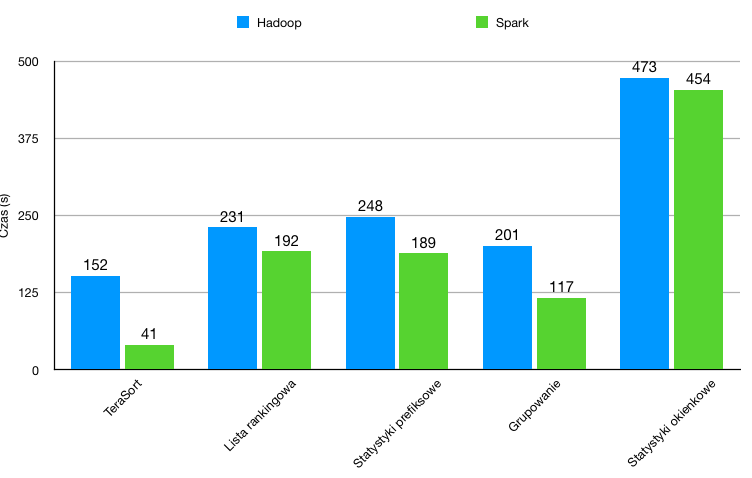
\includegraphics[width=13cm]{1_5_execution.png}
\end{figure}

\begin{figure}[H]
\centering
  \caption{Porównanie czasów wykonania algorytmów minimalnych na 5 GB danych przy użyciu 5 maszyn.}
  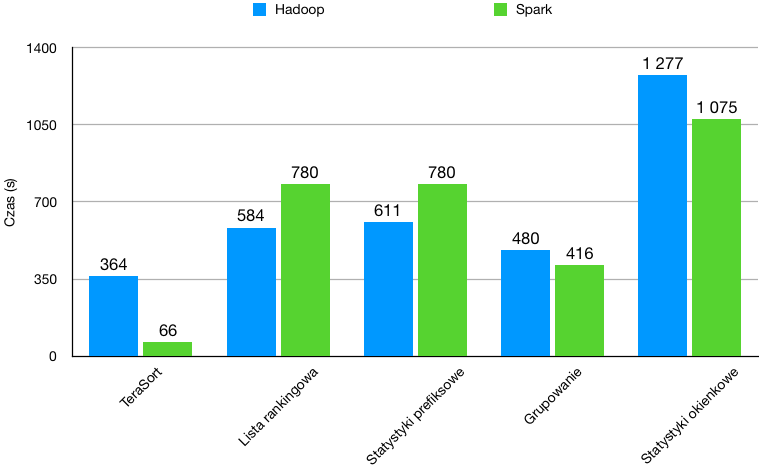
\includegraphics[width=13cm]{5_5_execution.png}
\end{figure}

\begin{figure}[H]
\centering
  \caption{Porównanie czasów wykonania algorytmów minimalnych na 1 GB danych przy użyciu 10 maszyn.}
  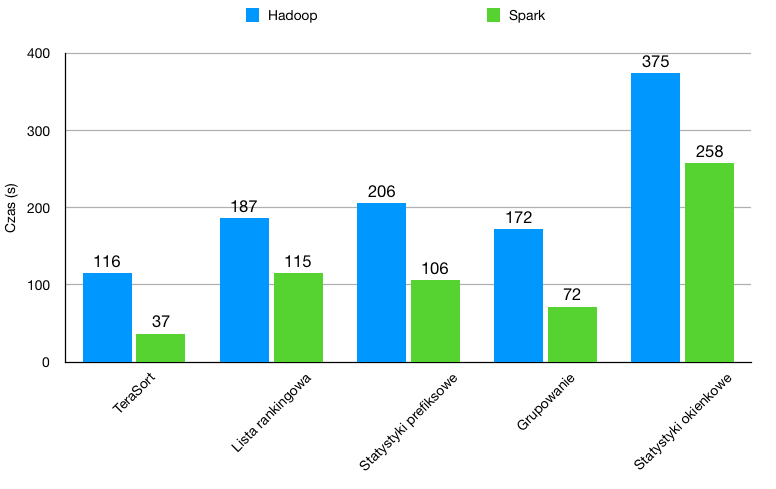
\includegraphics[width=13cm]{1_10_execution.png}
\end{figure}

\begin{figure}[H]
\centering
  \caption{Porównanie czasów wykonania algorytmów minimalnych na 5 GB danych przy użyciu 10 maszyn.}
  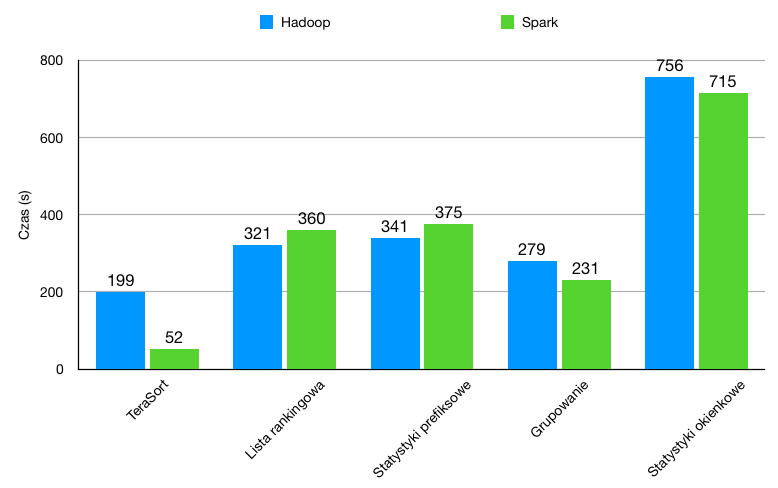
\includegraphics[width=13cm]{5_10_execution.png}
\end{figure}

Z wykresów wynika, że algorytm \textit{TeraSort} jest znacząco szybszy na Sparku. W implementacji Sparka \textit{grupowanie} oraz \textit{statystyka okienkowa} są zawsze szybsze, jednak \textit{lista rankingowa} oraz \textit{statystyki prefiksowe} niekoniecznie. Możemy zauważyć, że ilość danych wejściowych odgrywa bardzo ważną rolę. Przy rozmiarze 1 GB wszystkie algorytmy na Sparku są znacząco szybsze niż na Hadoopie. Natomiast przy wielkości 5 GB różnica maleje, a w przypadku \textit{listy rankingowej} oraz \textit{statystyk prefiksowych} Hadoop wygrywa. Powodem takiego zachowania jest zbyt mała ilość pamięci RAM na maszynach wchodzących w skład klastra. Jak wcześniej było wspomniane, Spark zawdzięcza swoją szybkość operacjom \textit{in-memory}. Niestety w przypadku zbyt małej ilości pamięci RAM, ta przewaga zostaje zniwelowana, a dodatkowo system musi zapisywać i odczytywać dane z dysku, tym samym tracąc swoją najcenniejszą właściwość.

\chapter{Podsumowanie}

Biblioteka algorytmów minimalnych powstała z myślą ułatwienia i przyspieszenia procesu tworzenia nowych algorytmów minimalnych oraz szybkiego dostępu do istniejących implementacji. W obecnych czasach programowanie rozproszone cały czas się rozwija i dlatego uważam, że biblioteka algorytmów minimalnych idealnie wpasowuje się w aktualny trend.

Impelementacja na Hadoopa wydaje się być dobrym narzędziem do używania, tworzenia i rozwijania algorytmów minimalnych. Posiada zwięzłe API oraz ułatwia korzystanie z paradygmatu MapReduce. Testy wypadły bardzo obiecująco. Niepokojące może być wysokie zużycie pamięci lokalnej maszyn. W przyszłości warto by powtórzyć testy, mierząc statystyki oddzielnie dla każdej maszyny wchodzącej w skład klastra. Dodatkowo warto przeprowadzić testy w warunkach identycznych do opisanych w pracy \cite{tao2013minimal}, a następnie porównać wyniki.

Rozwiązanie na Sparka, pod kątem użytkowalności, również wypada dobrze. Biblioteka jest łatwa i intuicyjna w użyciu. Niestety w aspekcie testów implementacja na Sparka prezentuje się nieco gorzej. Na podstawie przeprowadzonych testów można wyciągnąć wnioski, że biblioteka nie jest do końca zoptymalizowana. Przykład \textit{TeraSort} vs reszta algorytmów minimalnych pokazuje jak dużo można jeszcze osiągnąć. Należałoby jednak powtórzyć testy na klastrach złożonych z maszyn o większej ilości pamięci RAM.

Obecna wersja biblioteki nie jest jeszcze perfekcyjna, jednak stanowi bazę do rozpoczęcia kolejnych prac. Implementacje przykładowych algorytmów minimalnych oraz funkcji API spełniają warunki minimalności. Pozwala to optymistycznie patrzeć w przyszłość i zachęca do dalszego rozwoju biblioteki algorytmów minimalnych.

\bibliographystyle{plain}
\bibliography{refs.bib}


\end{document}


%%% Local Variables:
%%% mode: latex
%%% TeX-master: t
%%% coding: latin-2
%%% End:
